%\NeedsTeXFormat{LaTeX2e} 		%???

\documentclass[notheorems,12pt]{beamer}

\usepackage[czech]{babel}
\usepackage[utf8]{inputenc}
\usepackage[T1]{fontenc}
\usepackage{enumerate,epsf,colortbl,color,colordvi}
\usepackage{graphicx, float}
\usepackage{subfig} 	%subfloats.

\usetheme{metropolis}
\metroset{numbering=none}
%\usetheme{Berlin}
\usecolortheme{beaver}

\setbeamertemplate{itemize items}[square] % squares in itemize

% \setbeamertemplate{enumerate items}[square] % squares in enumerate
\setbeamercolor*{enumerate item}{fg=darkred}

% \setbeamertemplate{enumerate items}[square]
% \setbeamercolor{item projected}{bg=darkred,fg=black}
% \setbeamertemplate{enumerate item}{%
%   \usebeamercolor[bg]{item projected}%
%   \raisebox{1.3pt}{\colorbox{bg}{\color{fg}\footnotesize\insertenumlabel}}%
% }

\setbeamertemplate{theorems}[numbered]
\setbeamercovered{transparent} % transparent text after \pause
\setbeamercovered{again covered={\opaqueness<1->{15}}, dynamic} % makes part of the slide transparent

\usepackage{pifont} % pro pekne znacky http://ctan.org/pkg/pifont
\newcommand{\cmark}{\ding{51}} % pekne znacky
\newcommand{\xmark}{\ding{55}} % pekne zncky



\usepackage{graphicx}
\usepackage{amsmath}							% great math stuff
\usepackage{amsfonts}							% for blackboard bold, etc
\usepackage{amsthm}								% better theorem environments
\usepackage{amssymb}

\usepackage{units}
\usepackage{physics}
\usepackage{subfig} 	%subfloats.
\captionsetup[subfigure]{labelformat=empty} %odstrani (a), (b),... u subfloats

\usepackage{caption} %abych mohl pouzit \caption*{•}

\usefonttheme[onlymath]{serif} 	%dela peknou matematiku ;)


\nonumber
\title[]{\#filterbubble}
\date{}
\author{Františka Sandroni\\
        Jakub Dostál}
\institute{}
% ############################################
% ############################################
\begin{document}
\maketitle
% ############################################
% ############################################
\begin{frame}{Filter bubble}
    \center
    \vspace{-0.1cm}
    \begin{large}\textbf{Izolace od dostatečně širokého spektra informací.}\end{large}
    \vspace{0.8cm}
    \begin{columns}
    \column{5cm}
    \begin{itemize}
        \item sociální sítě
        \item preferenční algoritmy
        \item Eli Pariser (2011)
    \end{itemize}
    \column{6cm}
        \begin{figure}
            \centering
            % \subfloat{
\includegraphics[scale=0.035]{./Pics/fb.png}}\\
            
\includegraphics[scale=0.4]{./Pics/twitter.png}
        \end{figure}
    \end{columns}
\end{frame}
% ############################################
% ############################################
\begin{frame}{Filter bubble}
    \begin{columns}
    \column{5cm}
        \begin{block}{Problémy:}
    		\begin{itemize}
    			\item \textbf{homogenita} obsahu
                \item ztráta objektivity
                \item \textbf{radikalizace}
    		\end{itemize}
    	\end{block}
    \column{6cm}
    \begin{block}{Cíle:}
        \begin{itemize}
            \item metoda pro \textbf{studium} informační bubliny
            \item kvantitativní výzkum
            \item \textbf{detekce} filter bubble
        \end{itemize}
    \end{block}
    \end{columns}
\end{frame}
% ############################################
% ############################################
\begin{frame}{Metoda}
    \begin{enumerate}
        \begin{large}
        \onslide<1>\item\bfseries sběr dat
        \vspace{0.25cm}
        \onslide<0>\item výběr studované skupiny
        \vspace{0.25cm}
        \onslide<0>\item příspěvky sledované studovanými lidmi
        \vspace{0.25cm}
        \onslide<0>\item filtrace příspěvků na dané téma
        \vspace{0.25cm}
        \onslide<0>\item analýza vybraných příspěvků
        \vspace{0.25cm}
        \onslide<0>\item srovnání dat různých skupin
        \end{large}
    \end{enumerate}
\end{frame}
% ############################################
% ############################################
\begin{frame}{Twitter}
    \begin{columns}
    \column{5cm}
    	\begin{itemize}
    		\item sociální síť
    		\item informační kanál
            \item \textbf{following, followers}
    		\item Twitter API
    	\end{itemize}
    \column{6cm}
    	\center
    	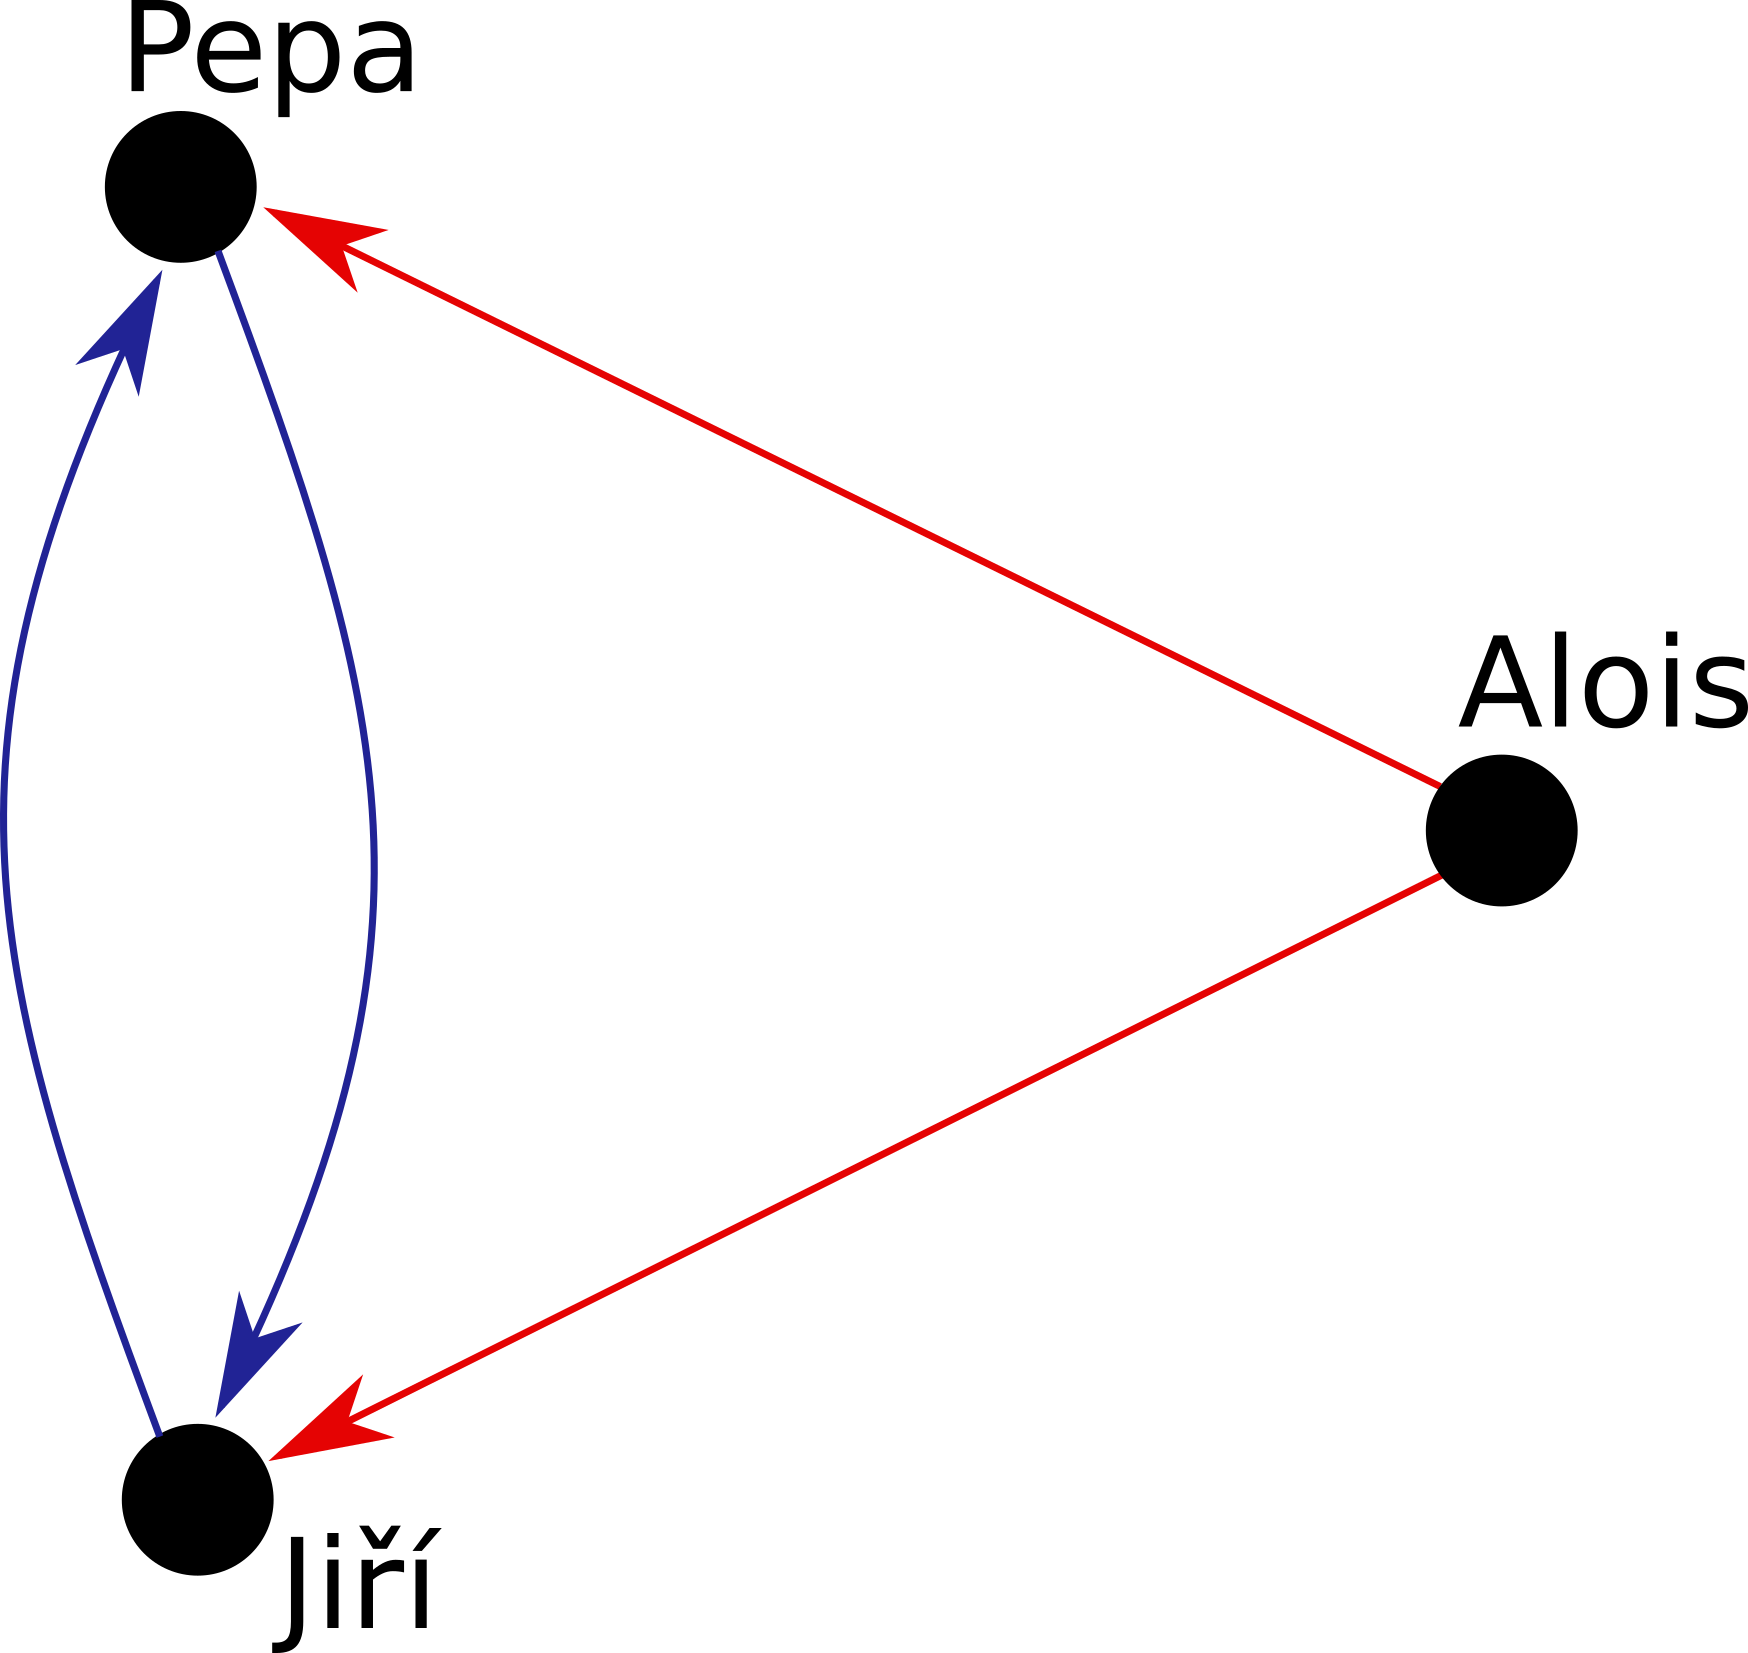
\includegraphics[scale=0.35]{./Pics/pepa.png}
    \end{columns}
\end{frame}
% ############################################
% ############################################
\begin{frame}{Metoda}
    \begin{enumerate}
        \begin{large}
        \onslide<1>\item sběr dat
        \vspace{0.25cm}
        \onslide<1>\item\bfseries výběr studované skupiny
        \vspace{0.25cm}
        \onslide<0>\item příspěvky sledované studovanými lidmi
        \vspace{0.25cm}
        \onslide<0>\item filtrace příspěvků na dané téma
        \vspace{0.25cm}
        \onslide<0>\item analýza vybraných příspěvků
        \vspace{0.25cm}
        \onslide<0>\item srovnání dat různých skupin
        \end{large}
    \end{enumerate}
\end{frame}
% ############################################
% ############################################
\begin{frame}{Výběr studované skupiny}
    \vspace{-0.7cm}
    \begin{columns}
    \column{5cm}
    	\begin{itemize}
    		\item pozorovaná skupina
    		\item \textbf{příslušnost ke komunitě}
    		\item náhodný výběr ze sledujících
    	\end{itemize}
    \column{6cm}
    	\center
    	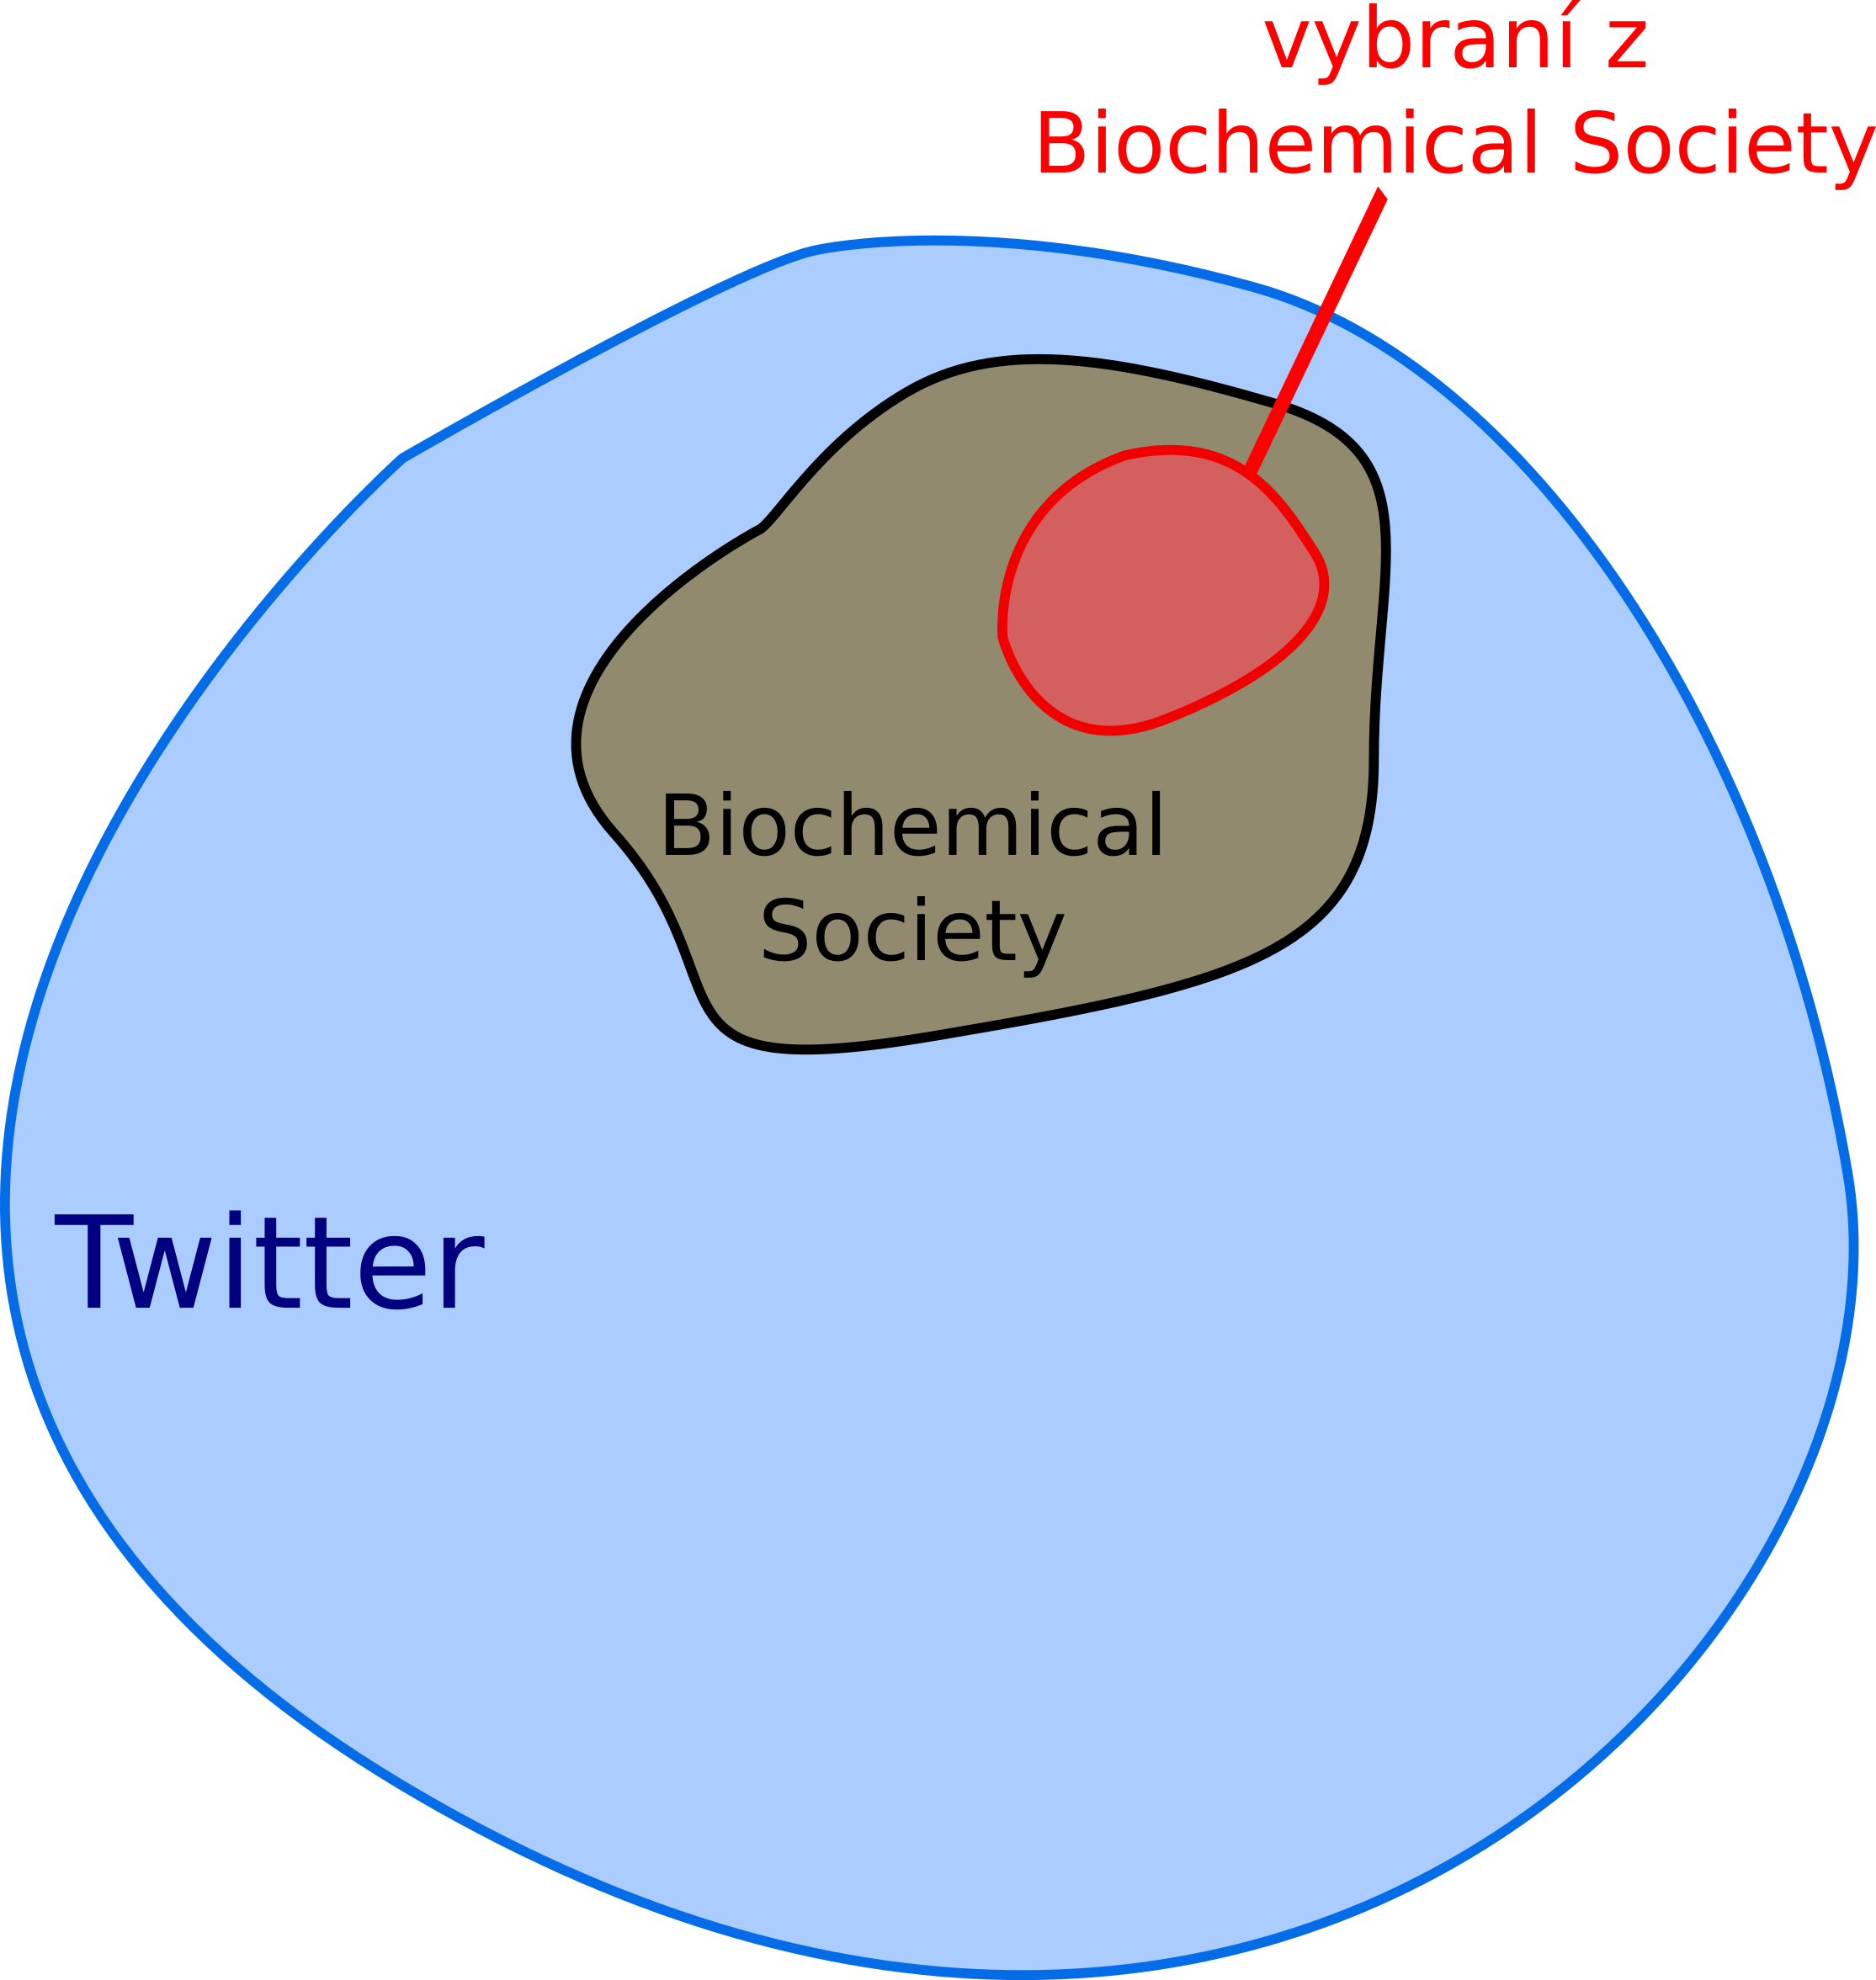
\includegraphics[scale=0.32]{./Pics/sets.png}
    \end{columns}
    \center
    \begin{large}
        $\text{Twitter} \rightarrow \text{Biochemical Society} \rightarrow \text{\textbf{studovaní lidé}}$
    \end{large}
\end{frame}
% ############################################
% ############################################
\begin{frame}{Metoda}
    \begin{enumerate}
        \begin{large}
        \onslide<1>\item sběr dat
        \vspace{0.25cm}
        \onslide<1>\item výběr studované skupiny
        \vspace{0.25cm}
        \onslide<1>\item\bfseries příspěvky sledované studovanými lidmi
        \vspace{0.25cm}
        \onslide<0>\item filtrace příspěvků na dané téma
        \vspace{0.25cm}
        \onslide<0>\item analýza vybraných příspěvků
        \vspace{0.25cm}
        \onslide<0>\item srovnání dat různých skupin
        \end{large}
    \end{enumerate}
\end{frame}
% ############################################
% ############################################
\begin{frame}{Sběr příspěvků}
    \begin{columns}
    \column{5cm}
    	\begin{itemize}
            \item příspěvky viditelné studovanými
    		\item \textbf{okolí uživatele}
    		\item vzájemné příspěvky
    	\end{itemize}
    \column{6cm}
    	\center
    	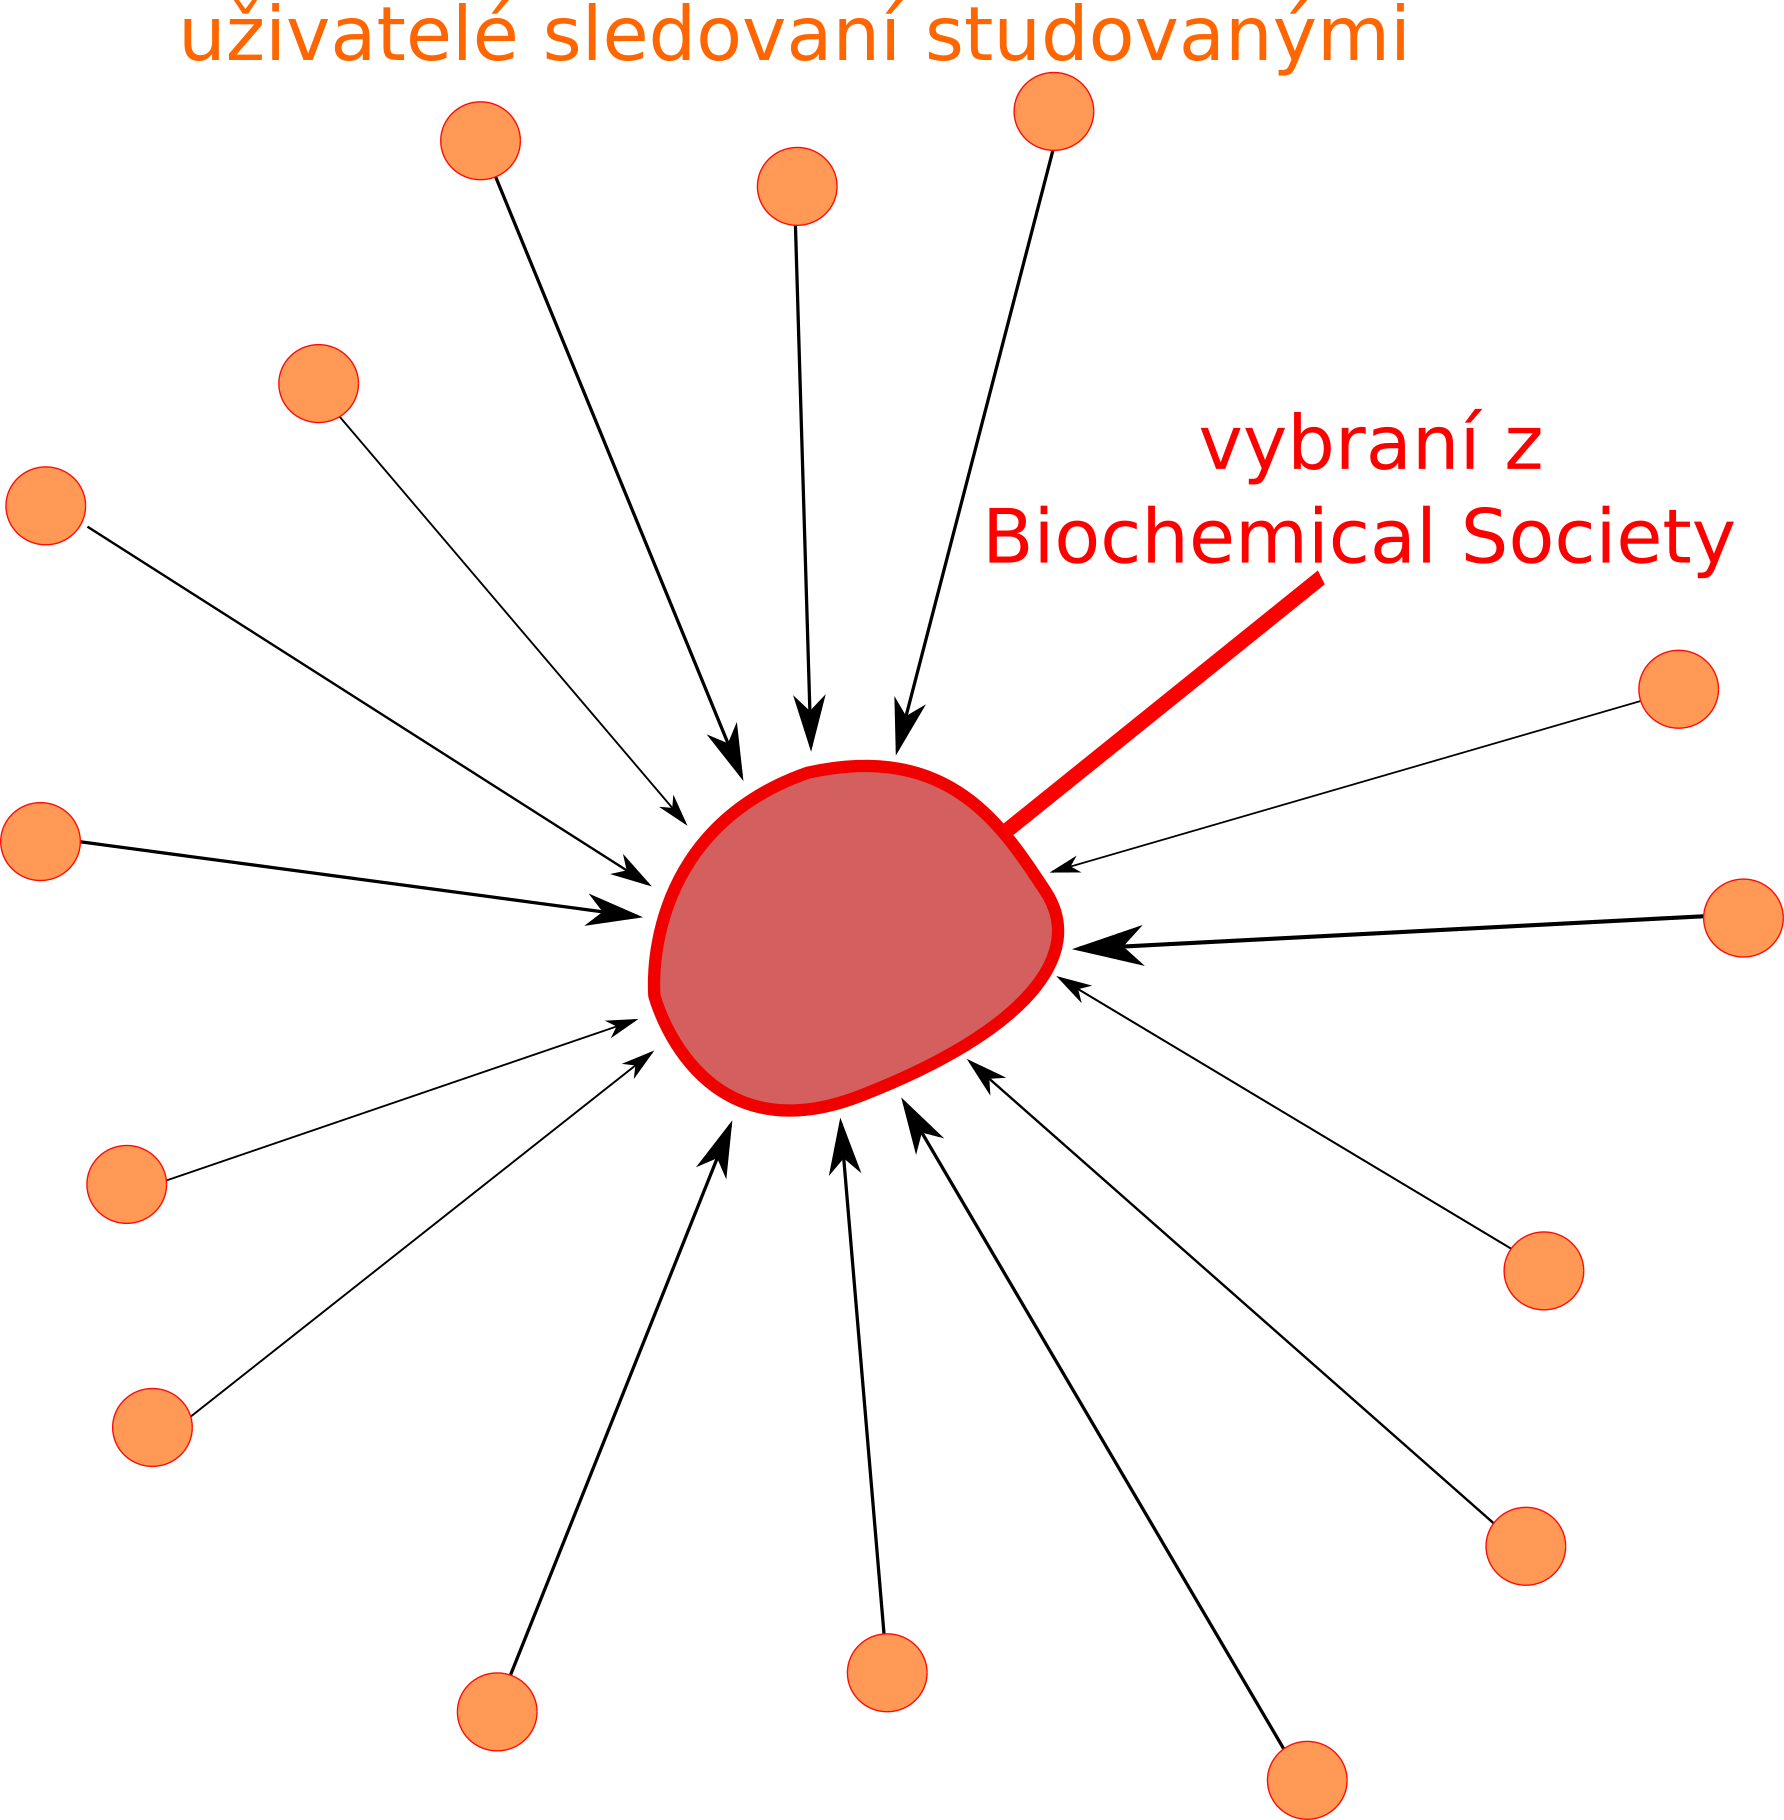
\includegraphics[scale=0.4]{./Pics/followers.png}
    \end{columns}
\end{frame}
% ############################################
% ############################################
\begin{frame}{Metoda}
    \begin{enumerate}
        \begin{large}
        \onslide<1>\item sběr dat
        \vspace{0.25cm}
        \onslide<1>\item výběr studované skupiny
        \vspace{0.25cm}
        \onslide<1>\item příspěvky sledované studovanými lidmi
        \vspace{0.25cm}
        \onslide<1>\item\bfseries filtrace příspěvků na dané téma
        \vspace{0.25cm}
        \onslide<0>\item analýza vybraných příspěvků
        \vspace{0.25cm}
        \onslide<0>\item srovnání dat různých skupin
        \end{large}
    \end{enumerate}
\end{frame}
% ############################################
% ############################################
\begin{frame}{Filtrace příspěvků}
\begin{itemize}
    \item přítomnost klíčového slova
    \item klíčové slovo = \textit{Trump}
\end{itemize}
% \vspace{0.7cm}
\center
Na snídani jsem měl vločky s mlékem. \xmark\\
\vspace{0.2cm}
Jsem velmi rád, že Donald \textbf{Trump} je prezidentem USA. \cmark\\
\vspace{0.2cm}
V USA mají nejlepšího prezidenta. \xmark\\
\end{frame}
% ############################################
% ############################################
\begin{frame}{Metoda}
    \begin{enumerate}
        \begin{large}
        \onslide<1>\item sběr dat
        \vspace{0.25cm}
        \onslide<1>\item výběr studované skupiny
        \vspace{0.25cm}
        \onslide<1>\item příspěvky sledované studovanými lidmi
        \vspace{0.25cm}
        \onslide<1>\item filtrace příspěvků na dané téma
        \vspace{0.25cm}
        \onslide<1>\item\bfseries analýza vybraných příspěvků
        \vspace{0.25cm}
        \onslide<0>\item srovnání dat různých skupin
        \end{large}
    \end{enumerate}
\end{frame}
% ############################################
% ############################################
\begin{frame}{Sentimentální analýza}
\begin{itemize}
    \item \textbf{positivní} vs. \textbf{negativní} text
    \item klasifikace
    \item machine learning, big data
\end{itemize}
% \vspace{0.7cm}
\center
\textit{Donald Trump je hrozný člověk.}\\
\textbf{(0.14)}\\
\vspace{0.5cm}
\textit{Donald Trump je skvělý člověk.}\\
\textbf{(0.95)}
\end{frame}
% ############################################
% ############################################
\begin{frame}{Metoda}
    \begin{enumerate}
        \begin{large}
        \onslide<1>\item sběr dat
        \vspace{0.25cm}
        \onslide<1>\item výběr studované skupiny
        \vspace{0.25cm}
        \onslide<1>\item příspěvky sledované studovanými lidmi
        \vspace{0.25cm}
        \onslide<1>\item filtrace příspěvků na dané téma
        \vspace{0.25cm}
        \onslide<1>\item analýza vybraných příspěvků
        \vspace{0.25cm}
        \onslide<1>\item\bfseries srovnání dat různých skupin
        \end{large}
    \end{enumerate}
\end{frame}
% ############################################
% ############################################
\begin{frame}{Klíčové slovo: Trump}
    \vspace{-1cm}
    \begin{figure}
        \centering
        \hspace{-0.5cm}
        \subfloat[]{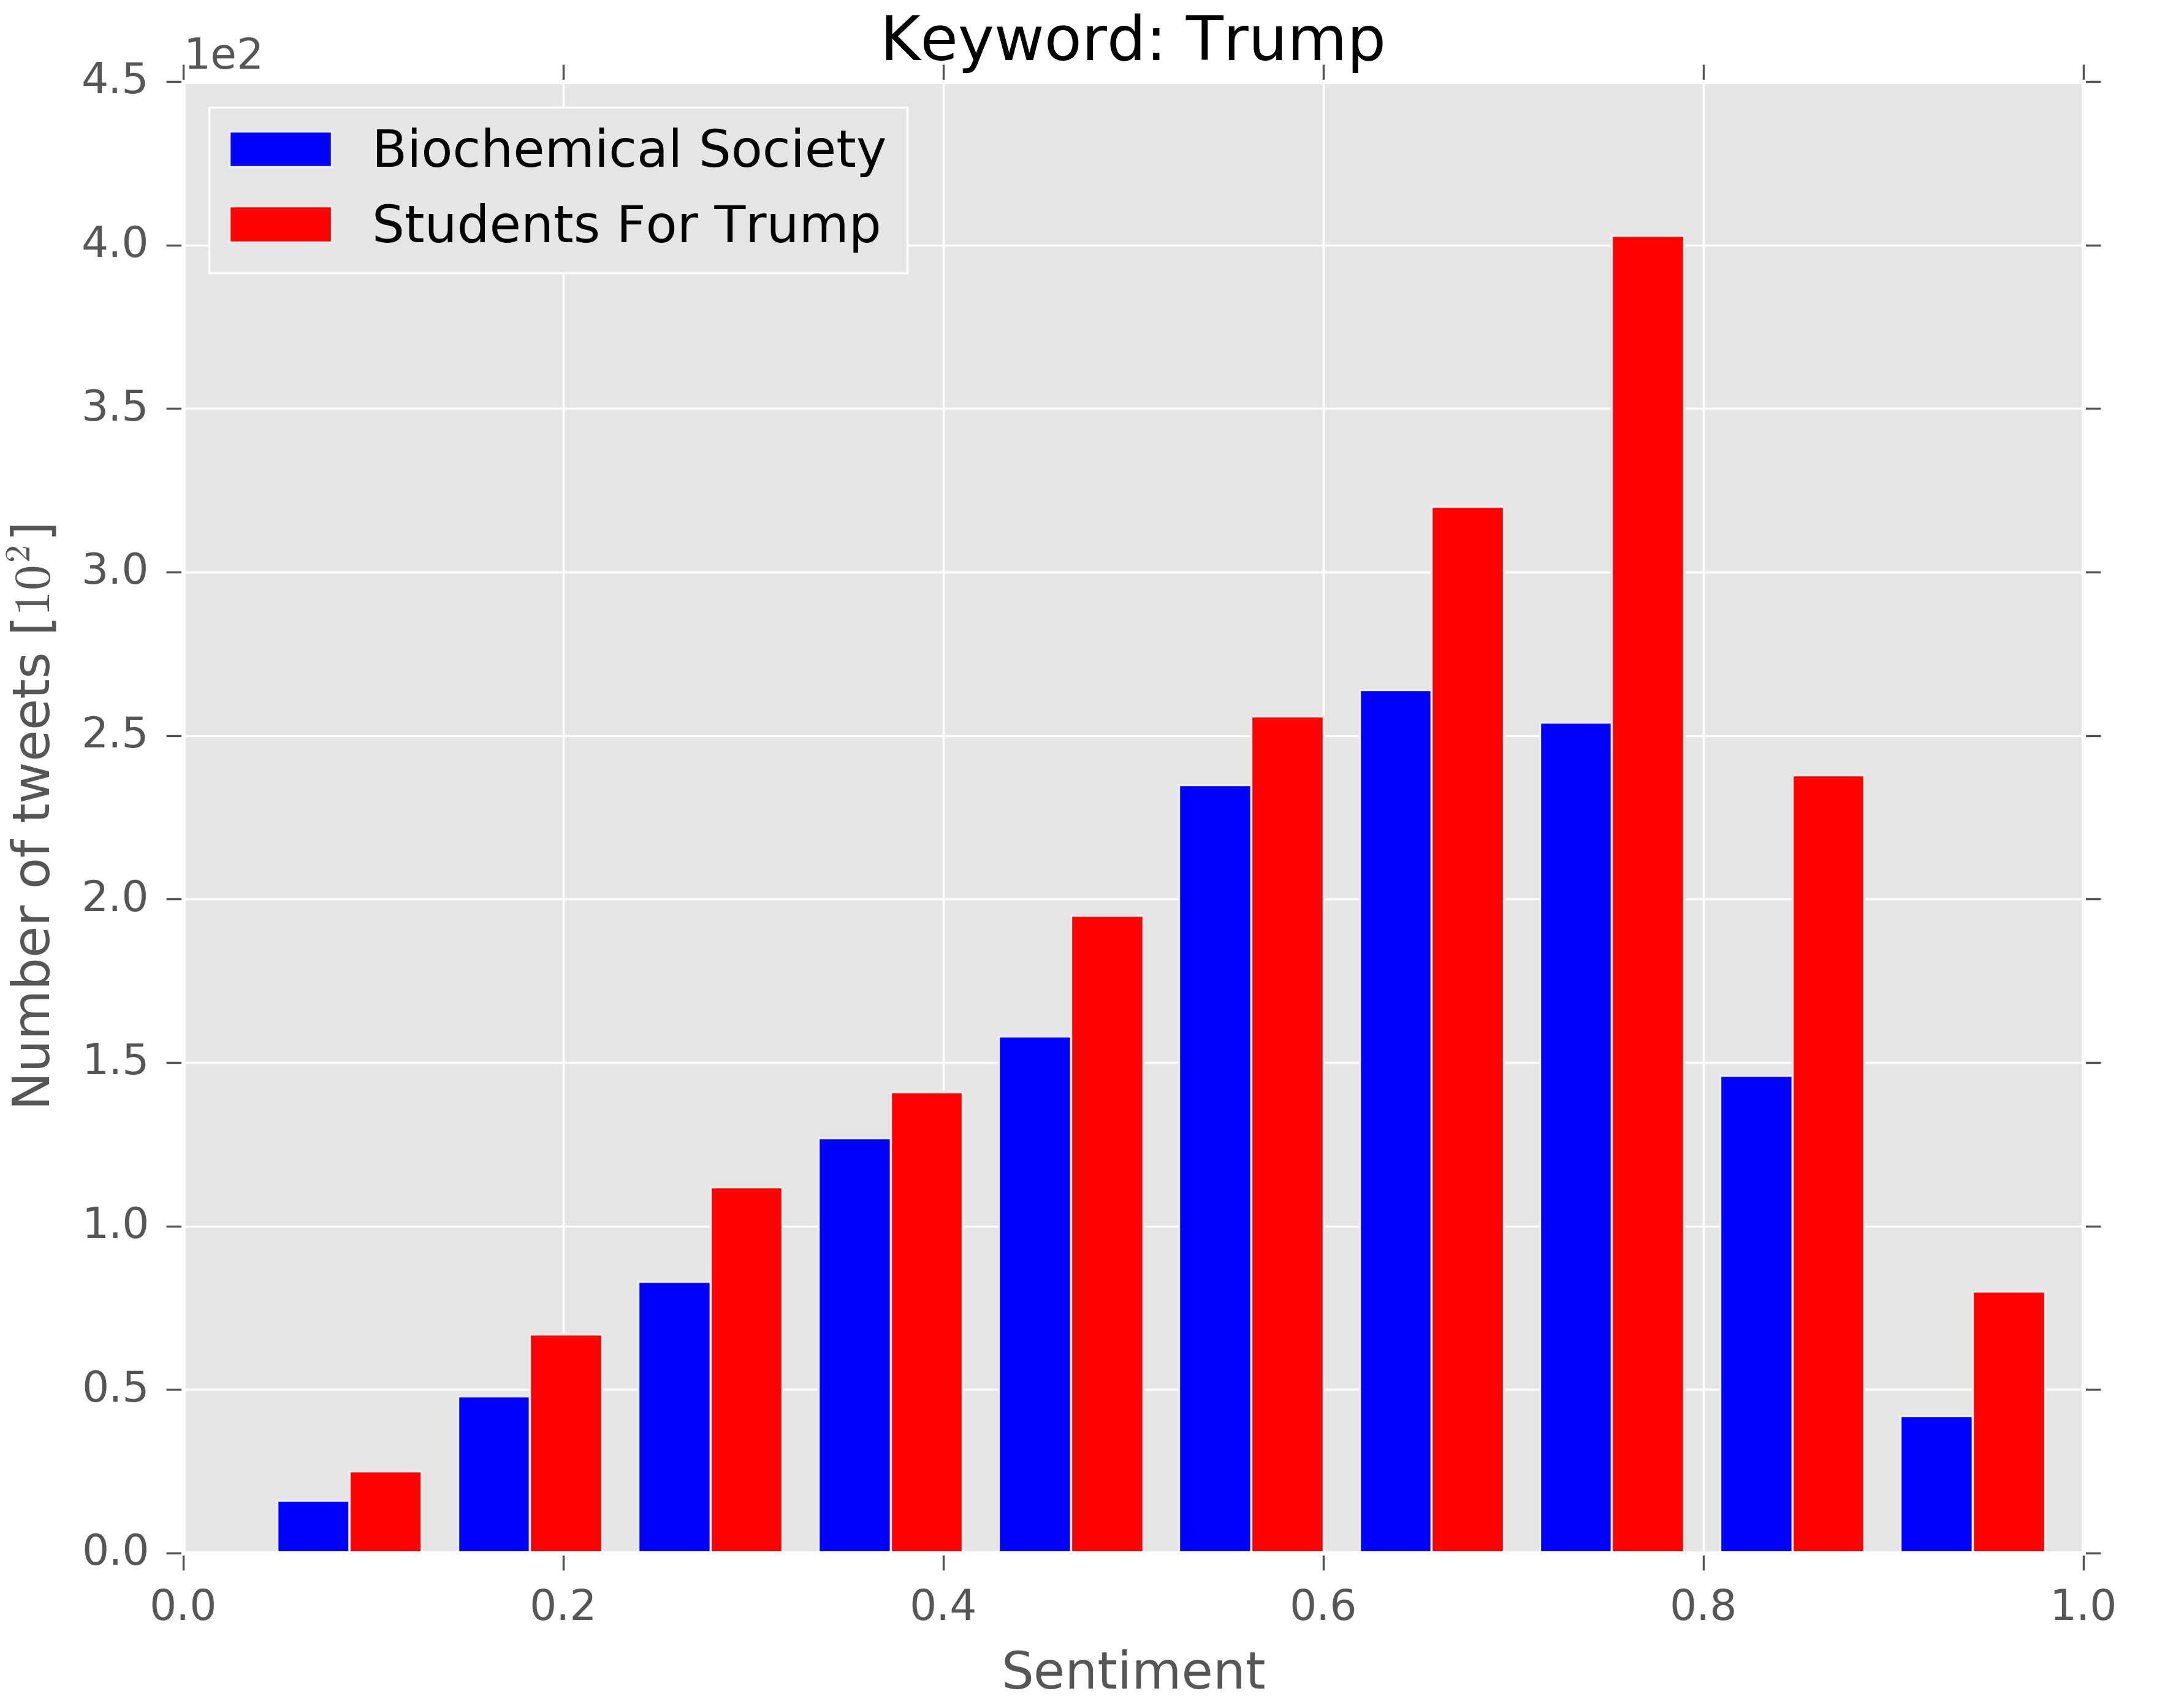
\includegraphics[scale=0.31]{./Pics/trump.png}}
        \subfloat[]{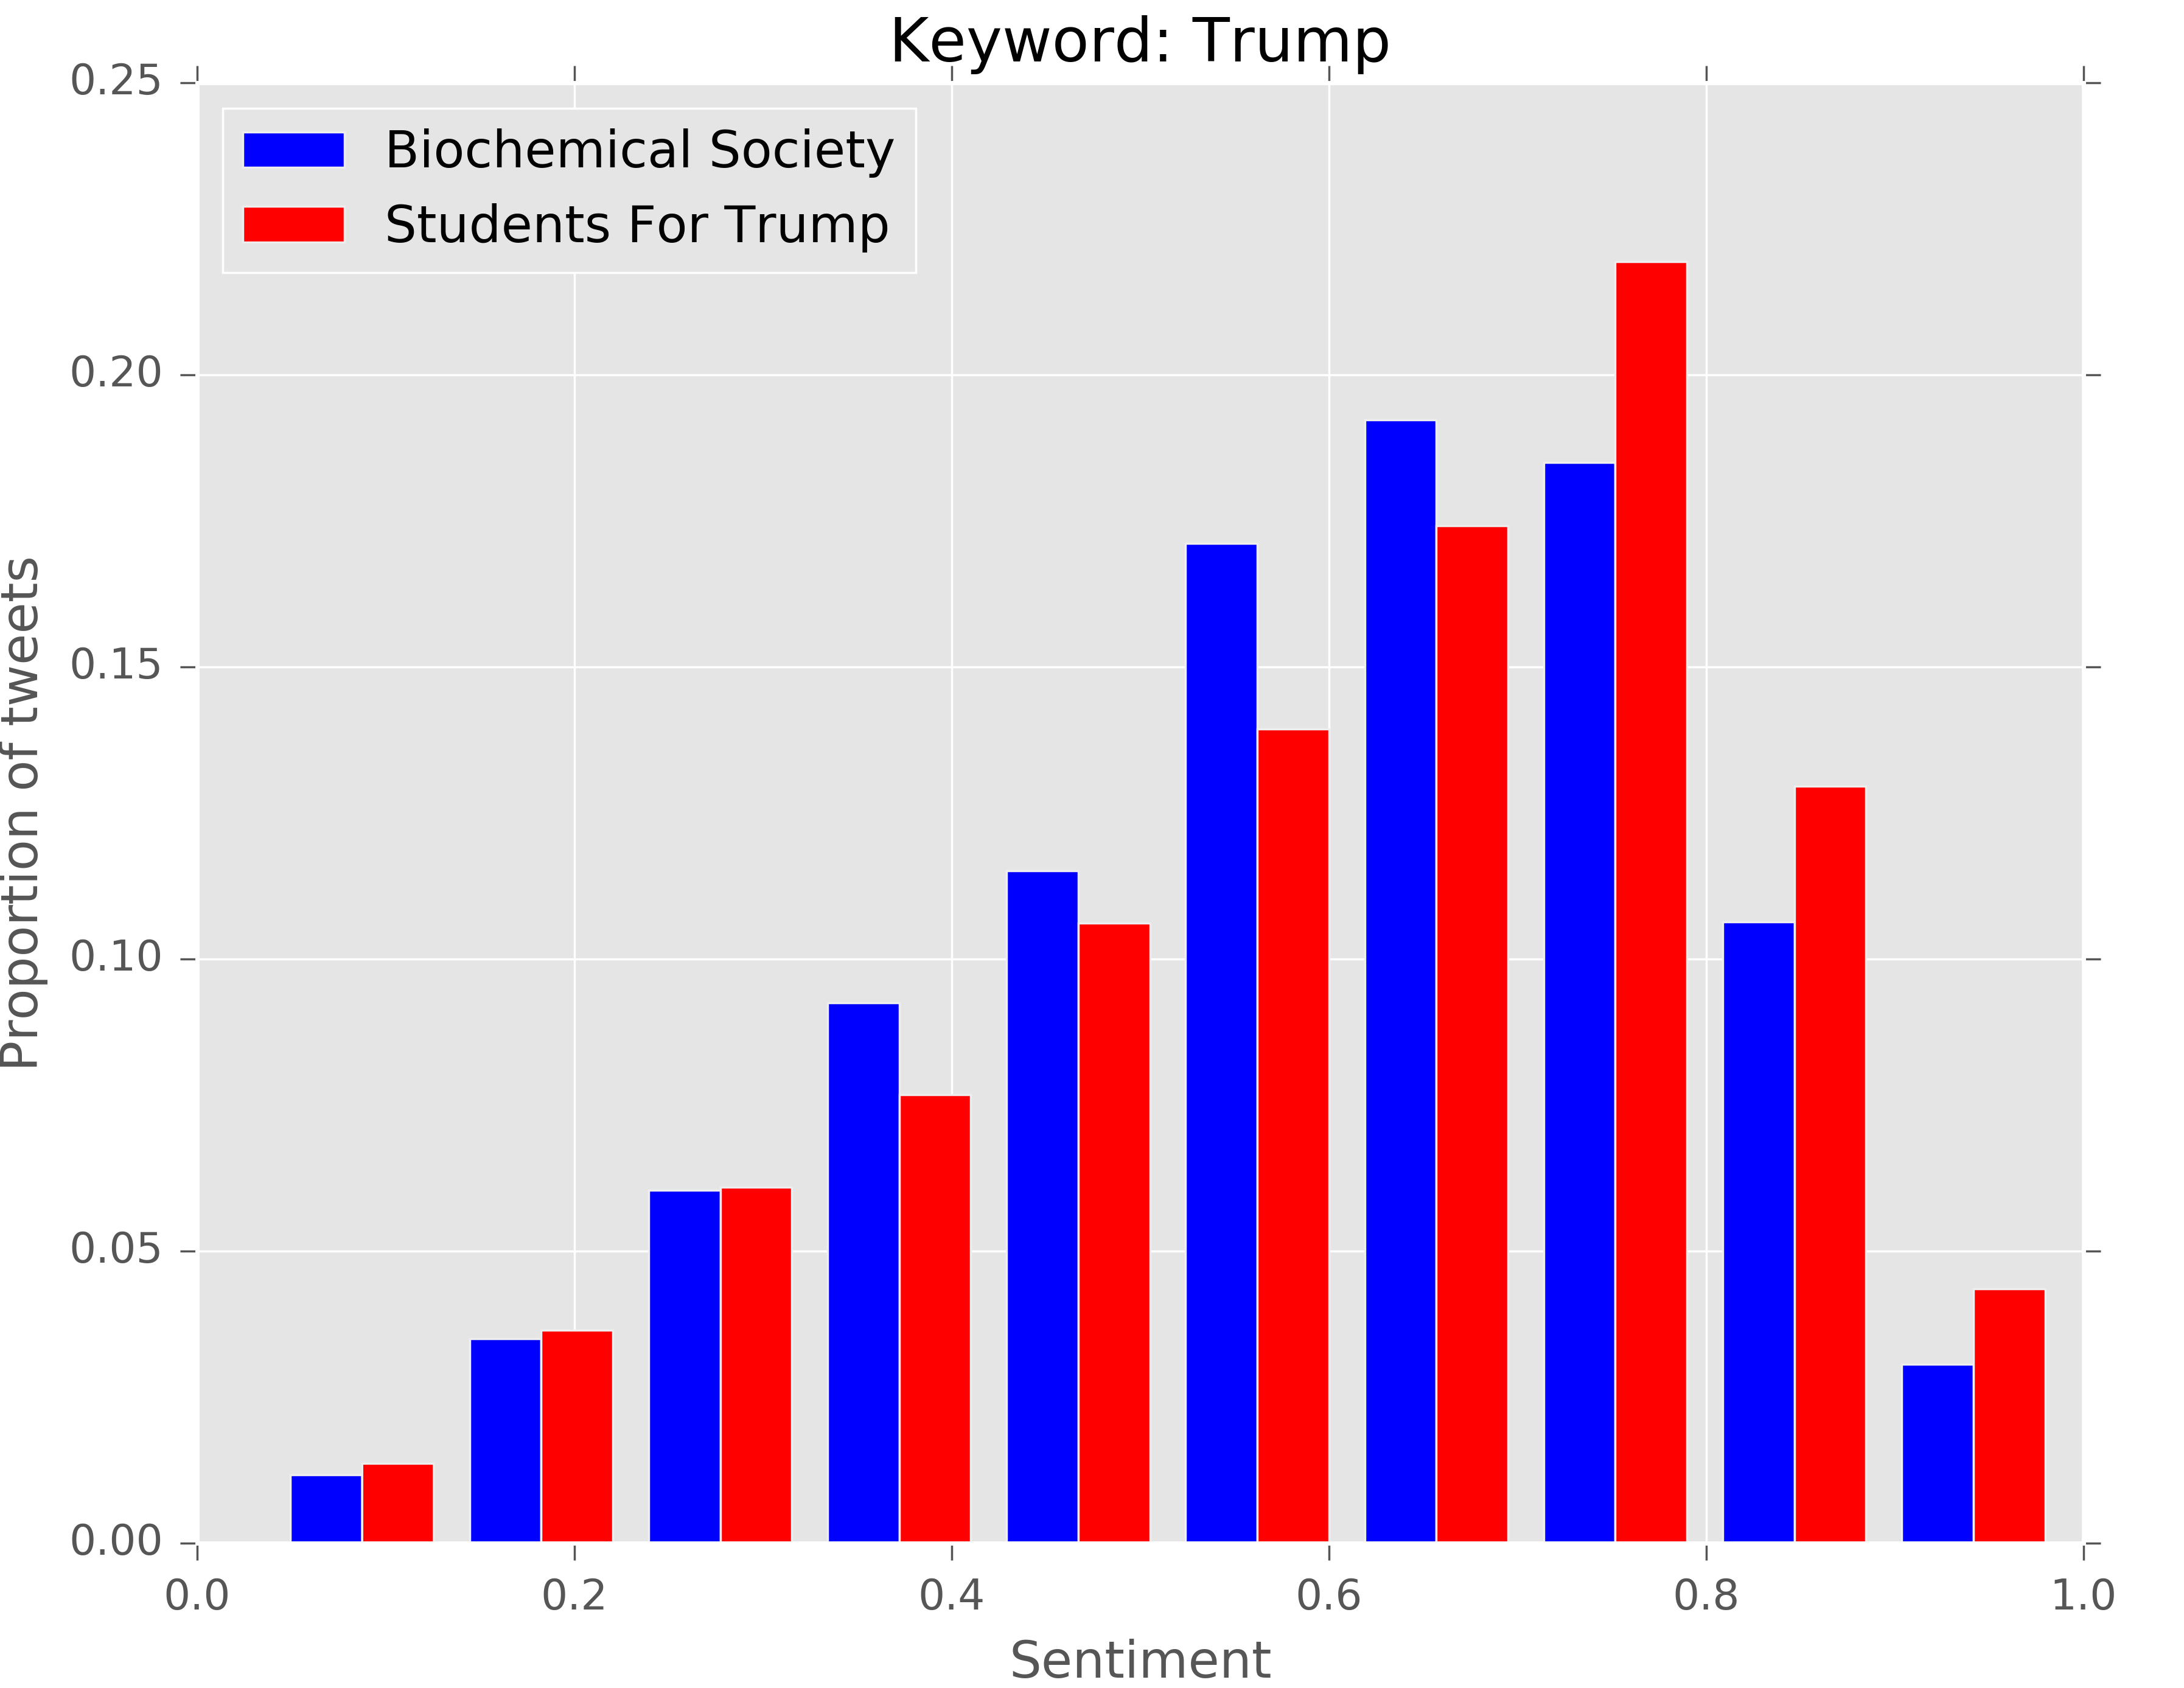
\includegraphics[scale=0.31]{./Pics/trump-normed.png}}
        \vspace{-0.7cm}
        \caption*{Histogramy počtu tweetů s klíčovým slovem \textit{\uv{Trump}}.}
    \end{figure}
	\begin{itemize}
		\item \textit{Biochemical Society} - financování vědy
		\item \textit{Students for Trump} - motivace
	\end{itemize}
\end{frame}
% ############################################
\begin{frame}{Klíčové slovo: Trump}
    \begin{figure}
        \centering
        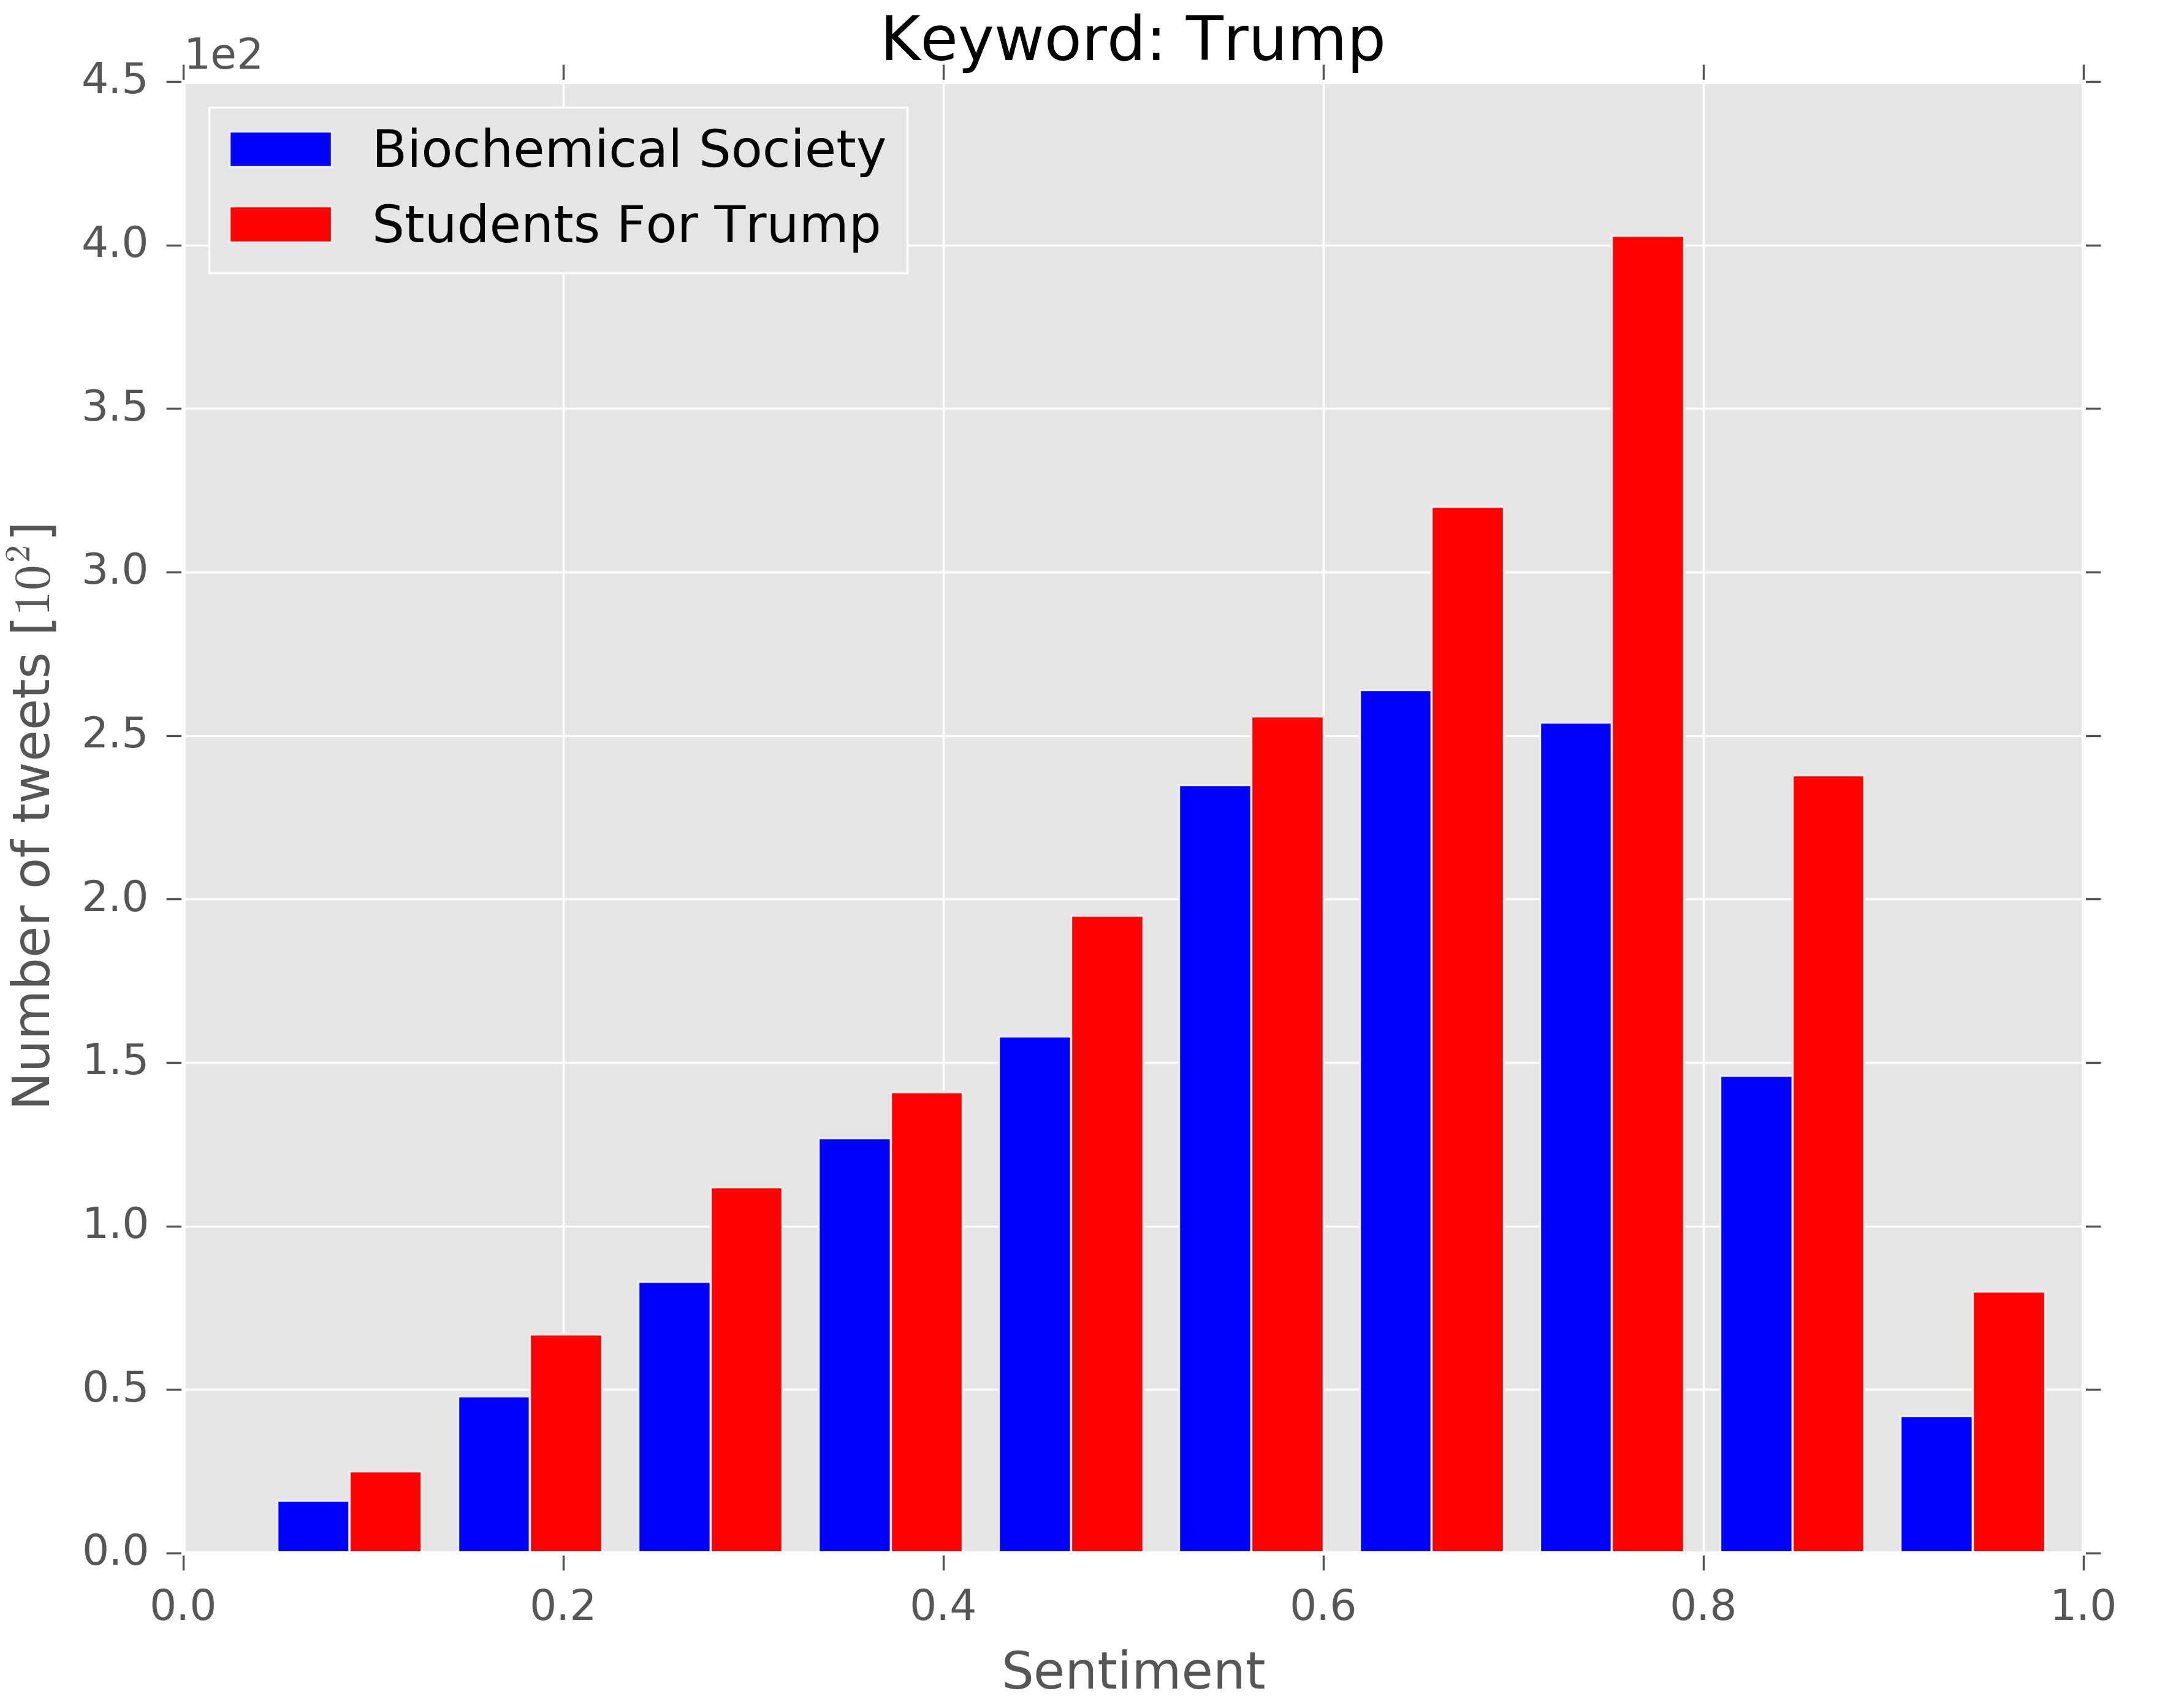
\includegraphics[scale=0.37]{./Pics/trump.png}
    \end{figure}
    \vspace{-0.4cm}
    \begin{itemize}
        \item \textbf{mírně rozdílný} počet příspěvků
        \item \textit{Students for Trump} spíše positivní
    \end{itemize}
\end{frame}
% ############################################
\begin{frame}{Klíčové slovo: Trump}
    \begin{figure}
        \centering
        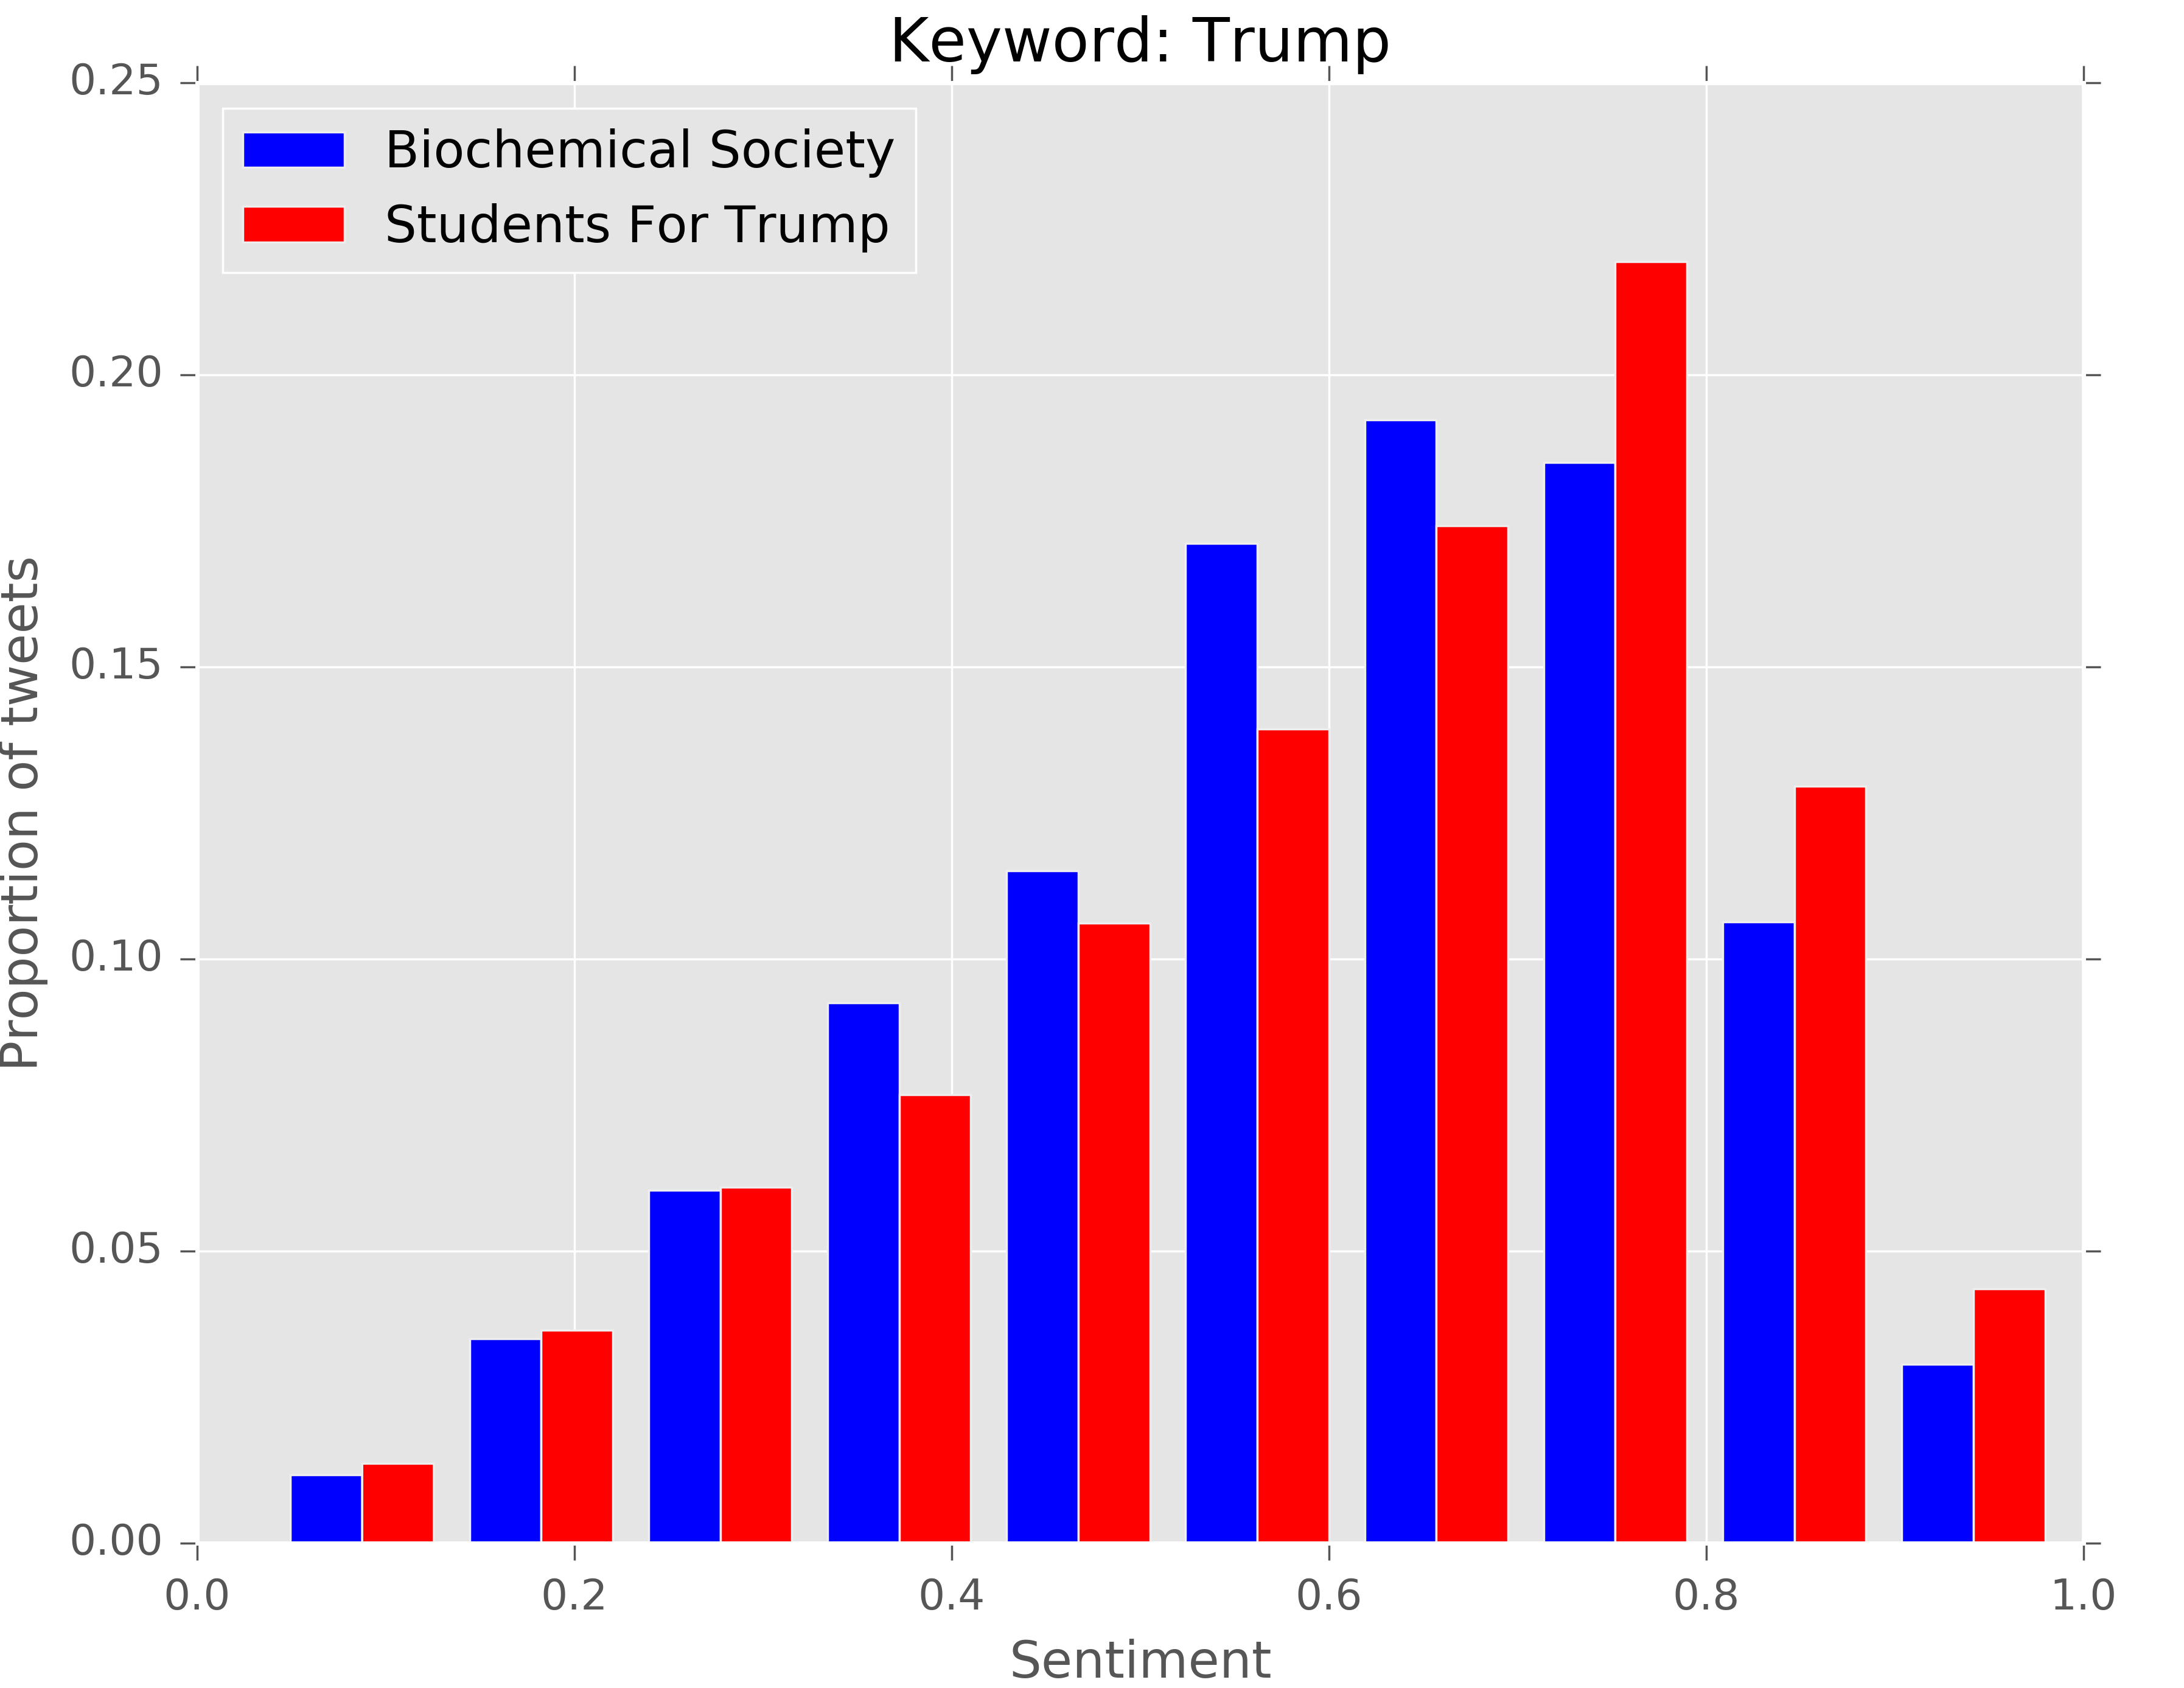
\includegraphics[scale=0.37]{./Pics/trump-normed.png}
        \vspace{-0.2cm}
        \caption*{Normalizovaný histogram - proporce sentimentu.}
    \end{figure}
    \vspace{-0.4cm}
	\begin{itemize}
        \item \textit{Biochemical Society} $\rightarrow$ sentiment $< 0.5$
		\item \textit{Students for Trump} $\rightarrow$ sentiment $> 0.5$
	\end{itemize}
\end{frame}
% ############################################
% ############################################
\begin{frame}{Klíčové slovo: potrat}
    \vspace{-1cm}
    \begin{figure}
        \centering
        \hspace{-0.5cm}
        \subfloat[]{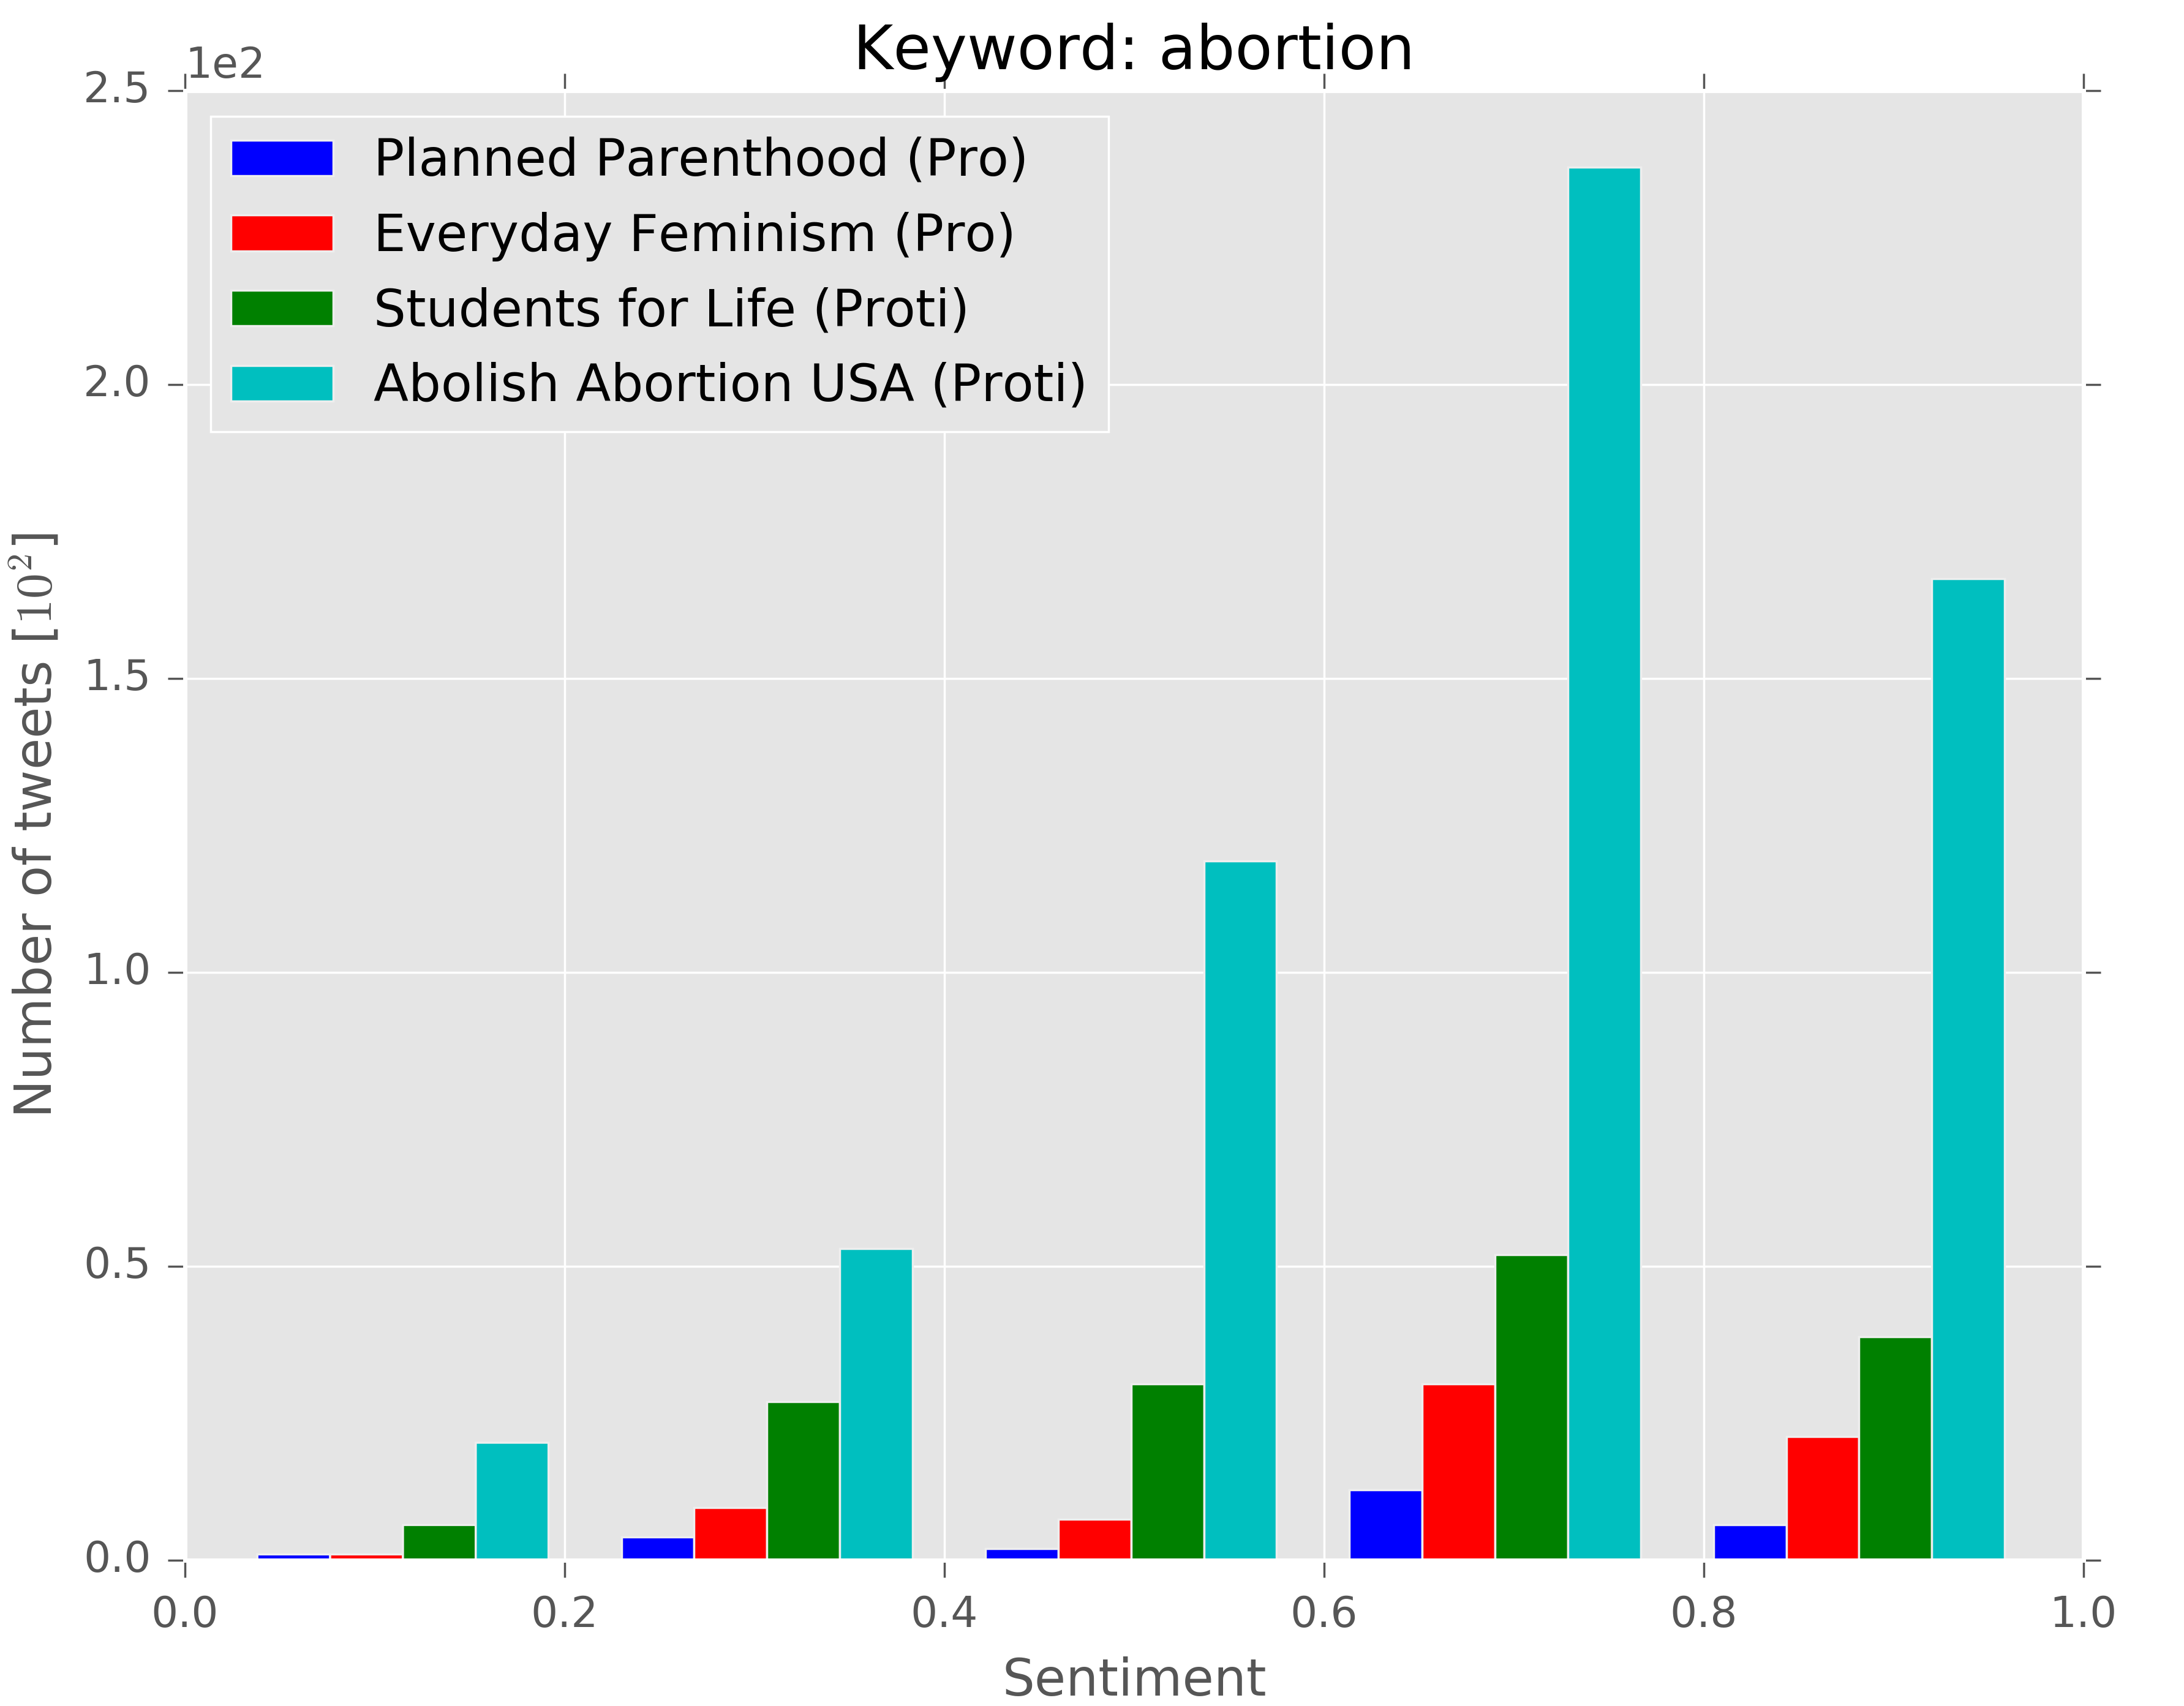
\includegraphics[scale=0.31]{./Pics/abortion.png}}
        \subfloat[]{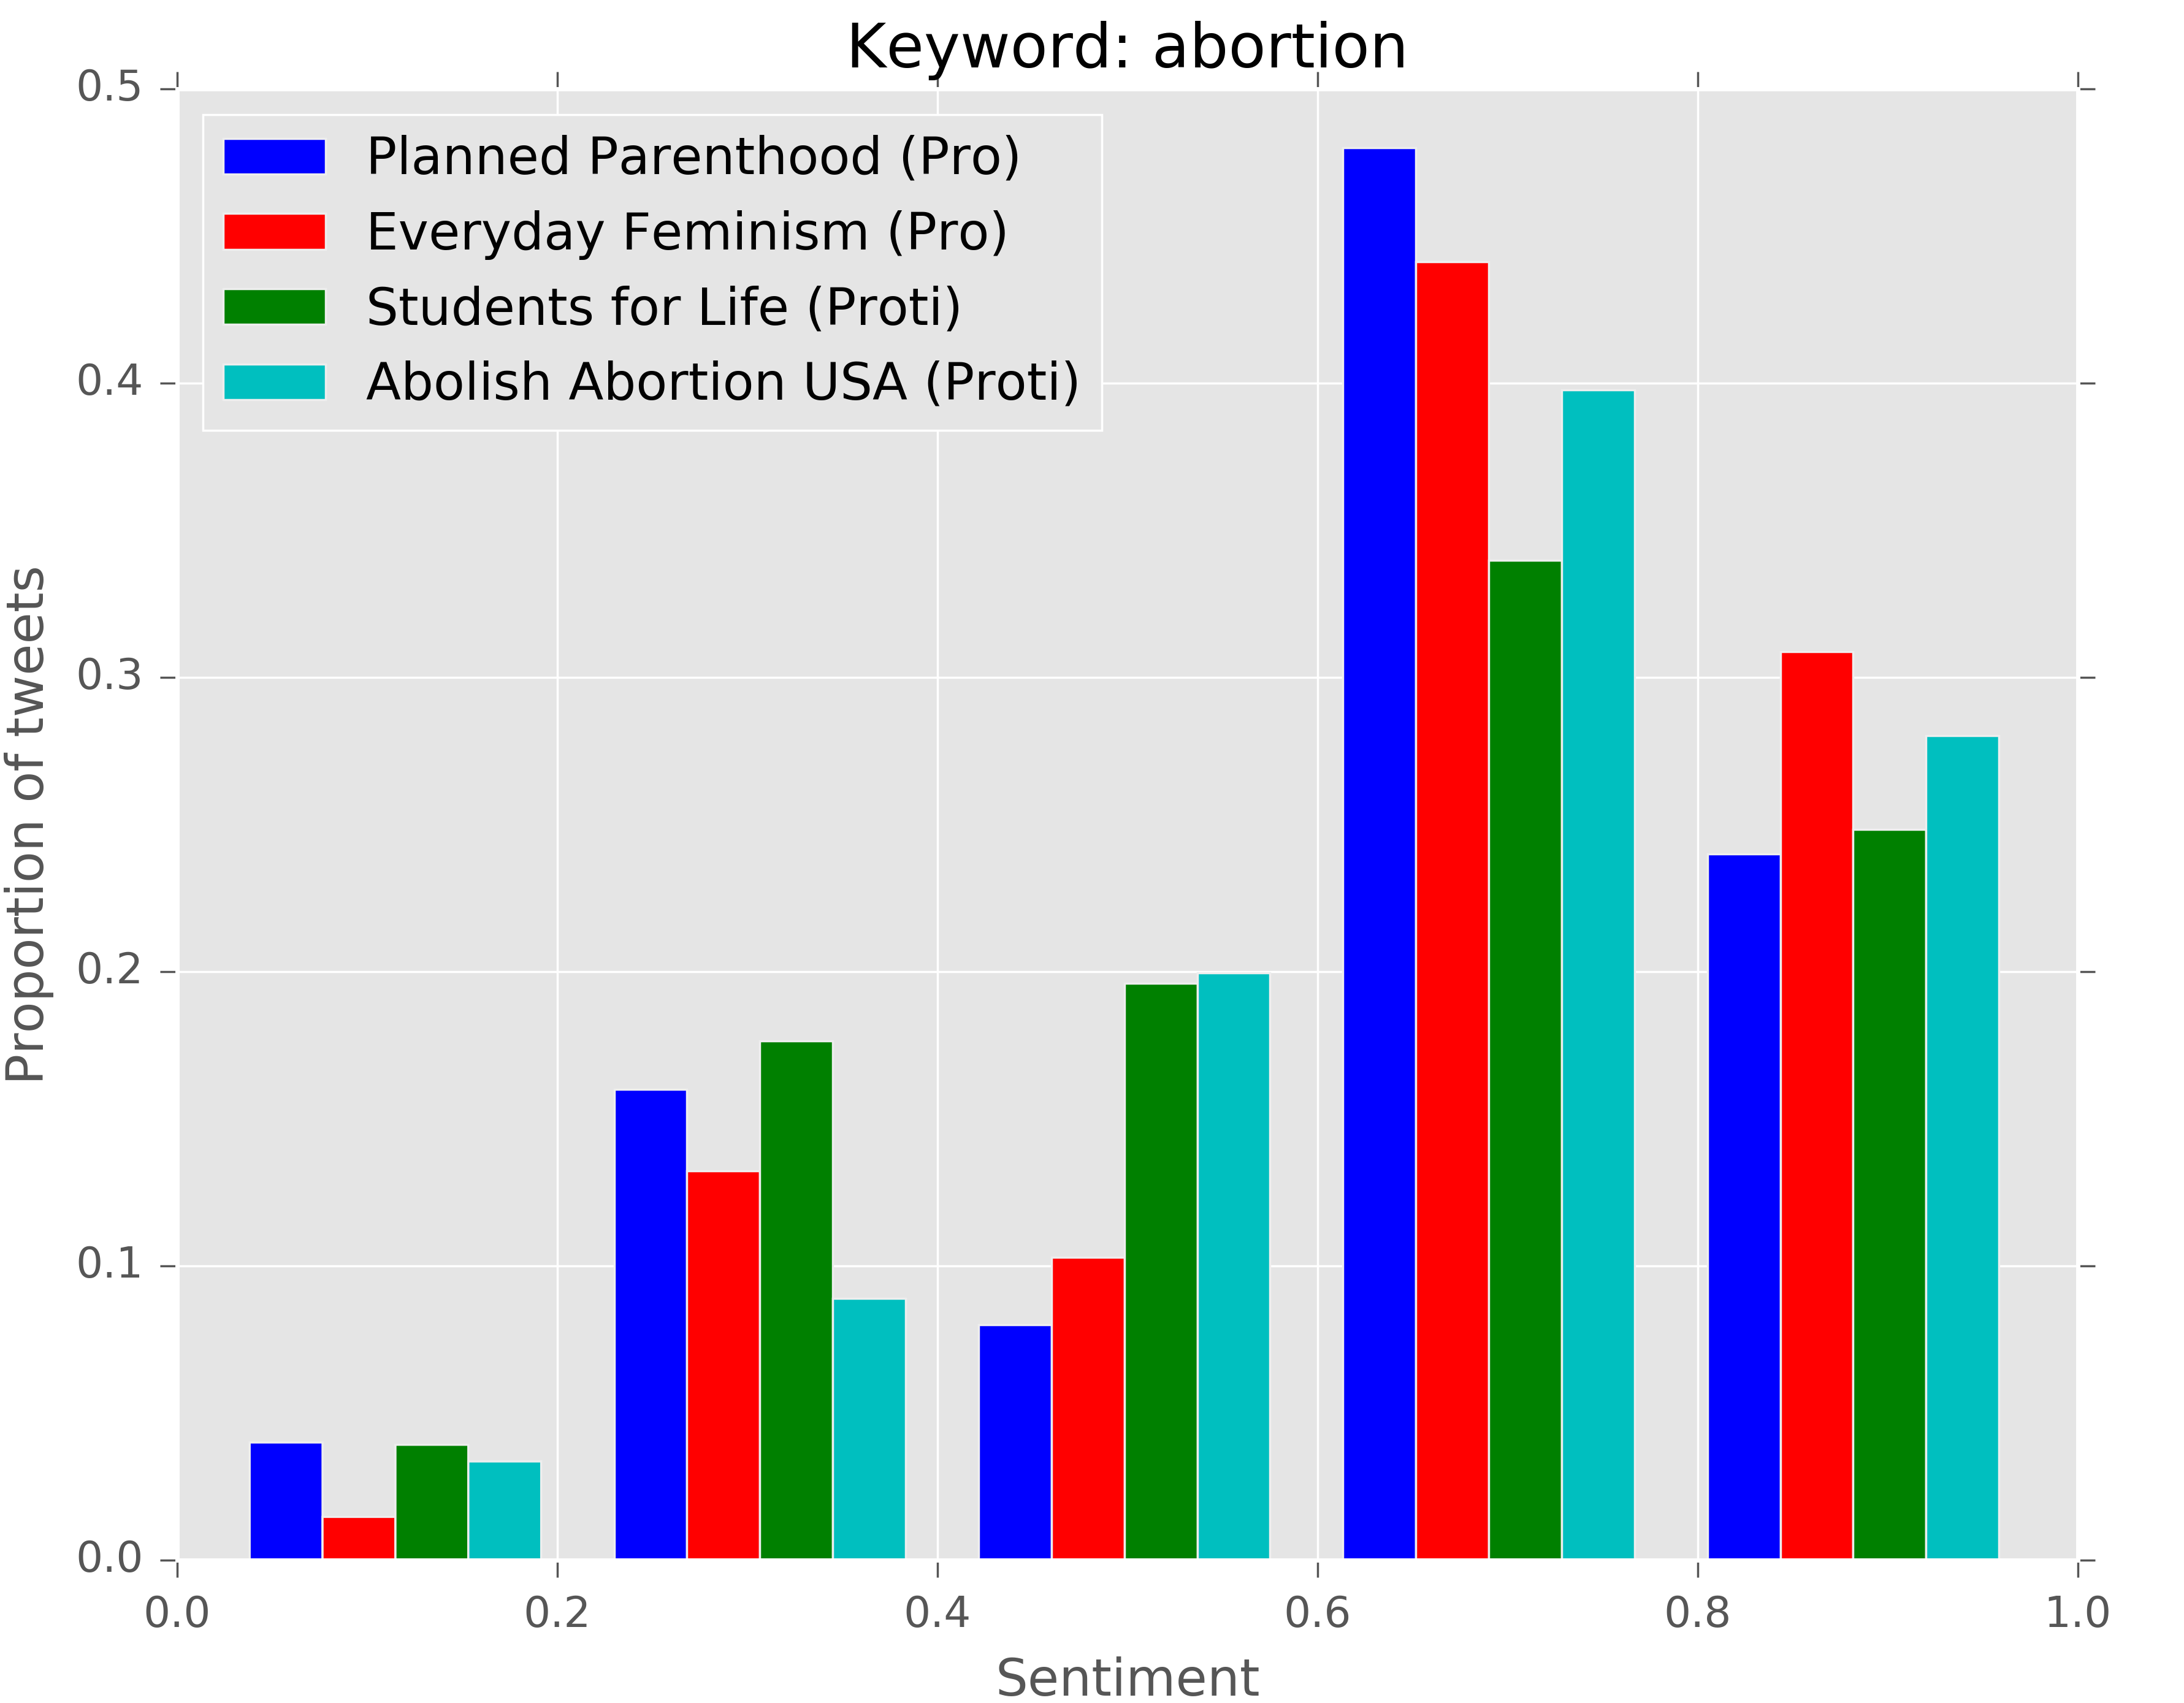
\includegraphics[scale=0.31]{./Pics/abortion-normed.png}}
        \vspace{-0.7cm}
        \caption*{Histogramy počtu tweetů s klíčovým slovem \textit{\uv{abortion}}.}
    \end{figure}
    \vspace{-0.3cm}
    \begin{columns}
    \column{6cm}
    	\begin{itemize}
    		\item \textit{Planned Parenthood}
    		\item \textit{Everyday Feminism}
    	\end{itemize}
    \column{6cm}
    	\begin{itemize}
    		\item \textit{Student for Life}
    		\item \textit{Abolish Abortion USA}
    	\end{itemize}
    \end{columns}
\end{frame}
% ############################################
\begin{frame}{Klíčové slovo: potrat}
    \begin{figure}
        \centering
        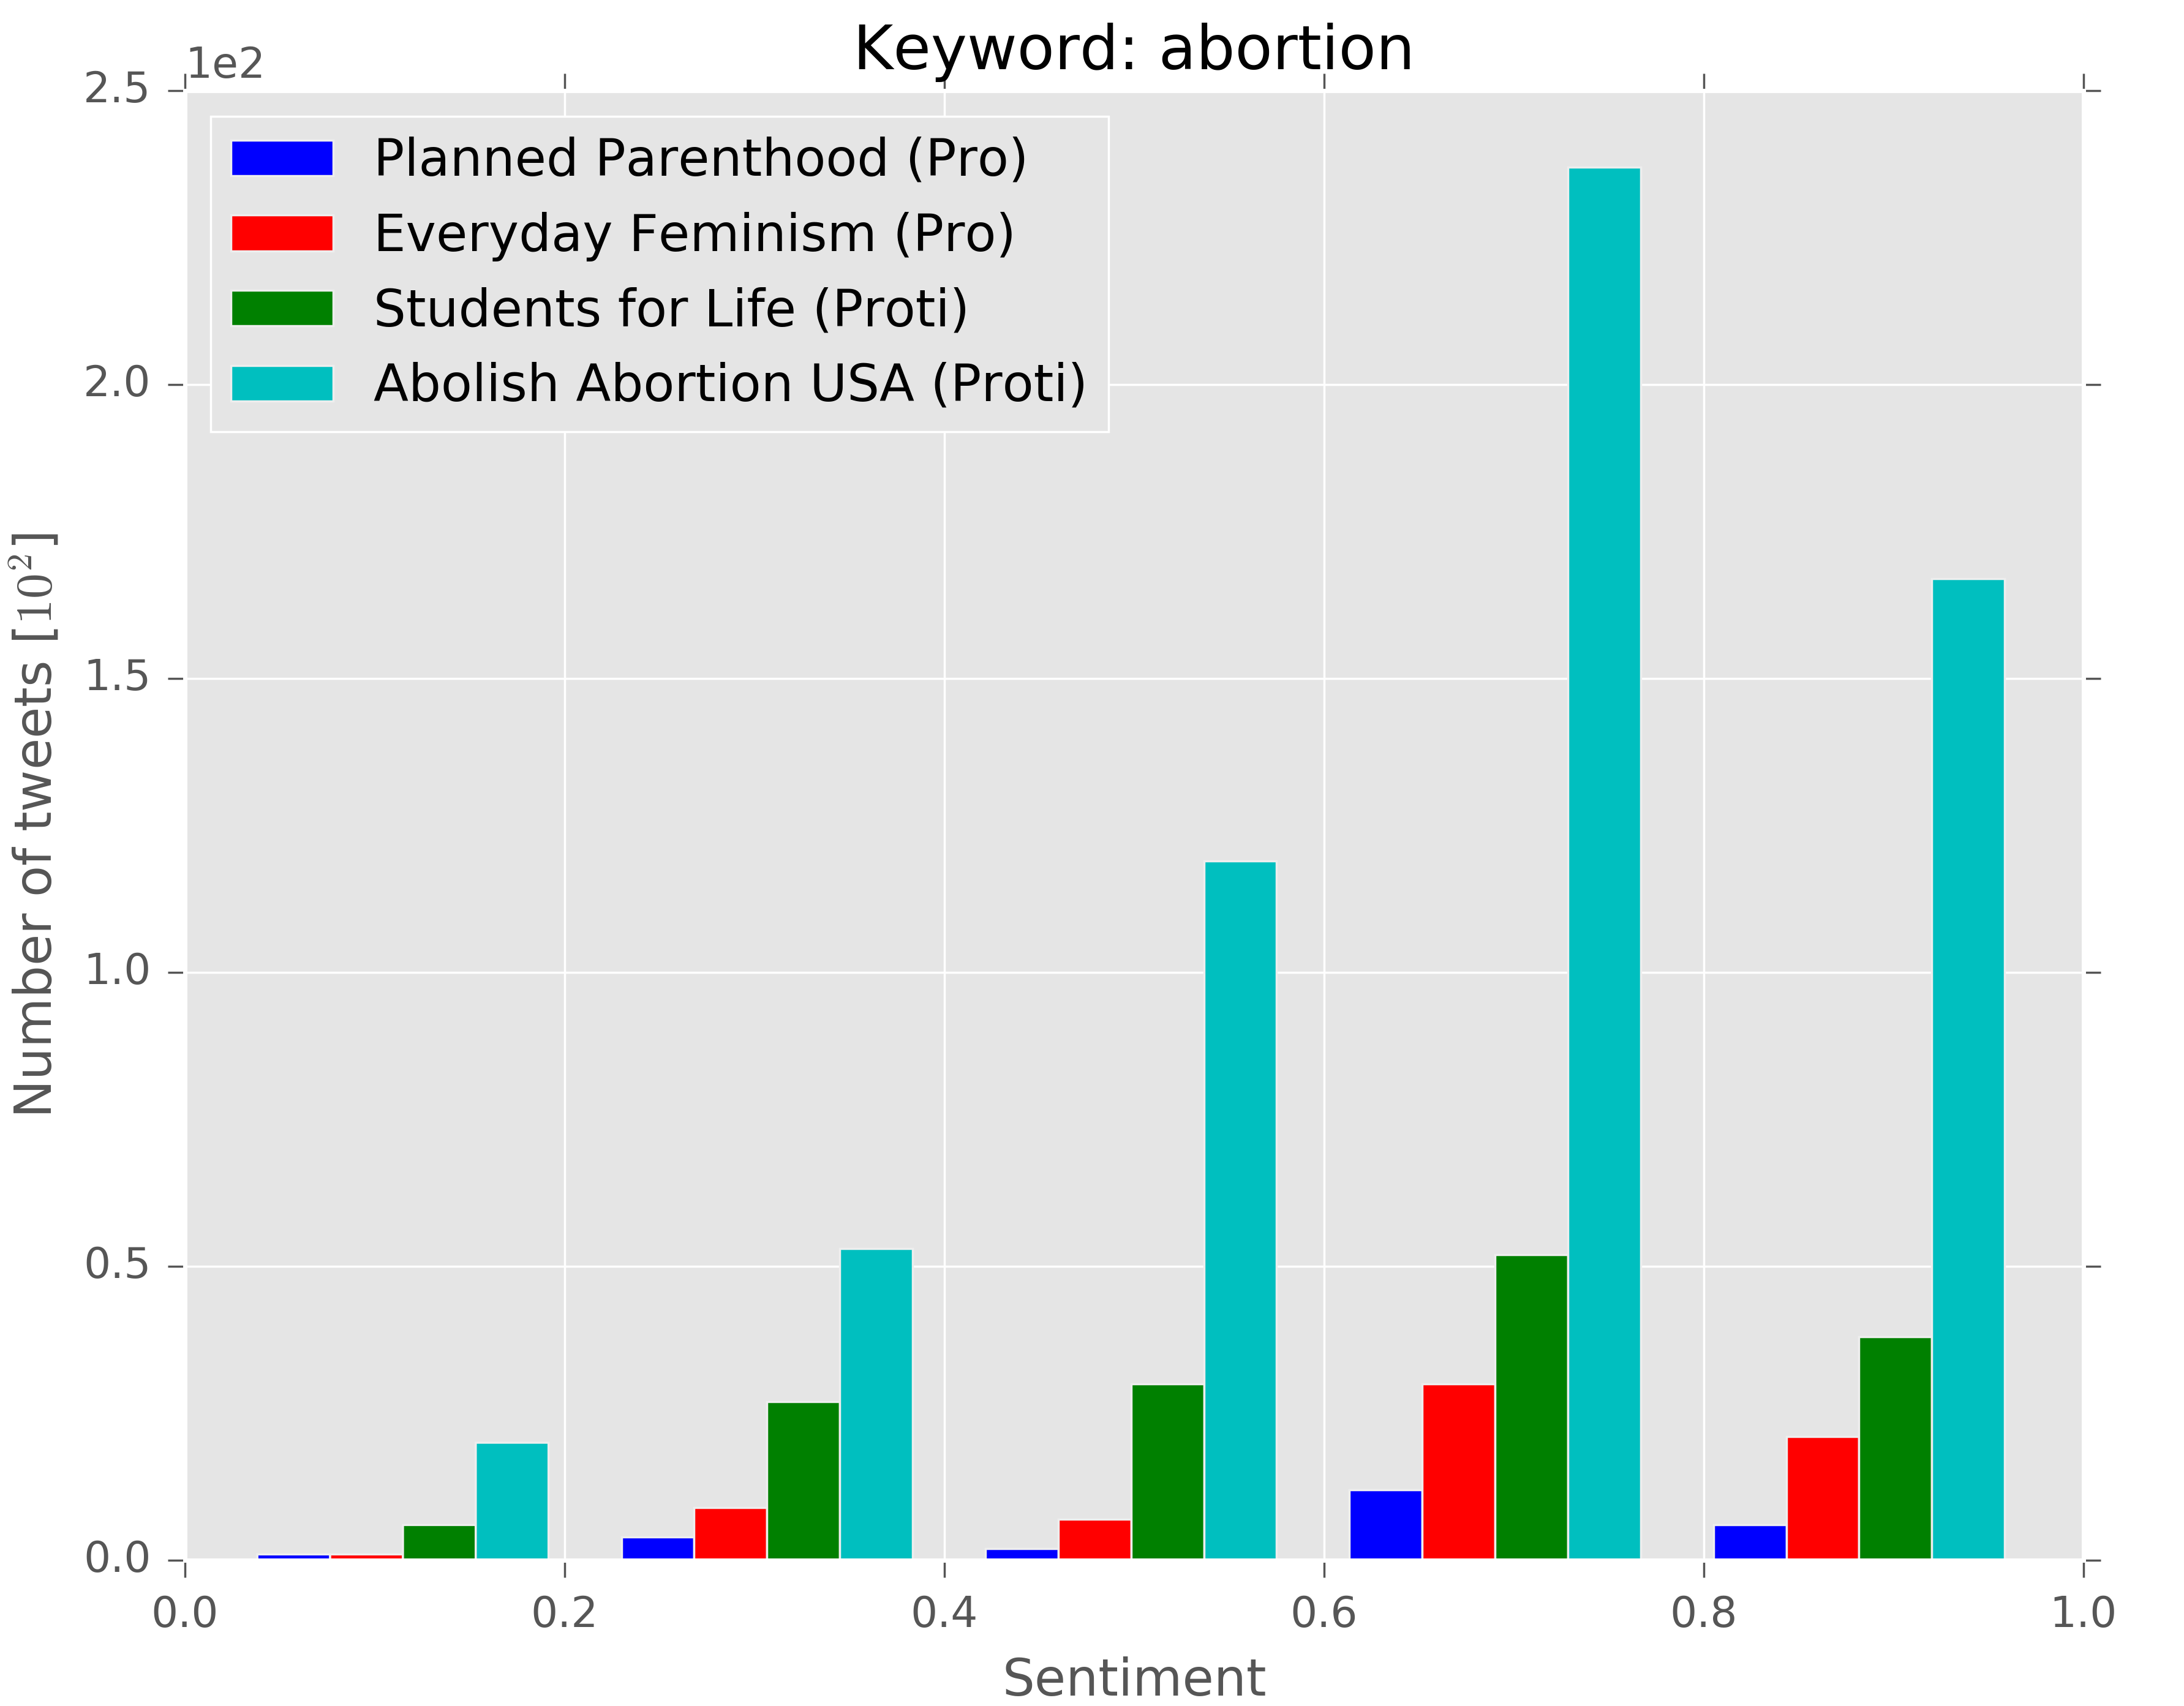
\includegraphics[scale=0.37]{./Pics/abortion.png}
    \end{figure}
    \vspace{-0.4cm}
    \begin{columns}
    \column{6cm}
    	\begin{itemize}
    		\item velký rozdíl v počtu tweetů
            \item objektivita je ohrožena
    	\end{itemize}
    \column{6cm}
    	\begin{itemize}
    		\item \textbf{větší aktivita} skupin proti potratu
    	\end{itemize}
    \end{columns}
\end{frame}
% ############################################
\begin{frame}{Klíčové slovo: potrat}
    \begin{figure}
        \centering
        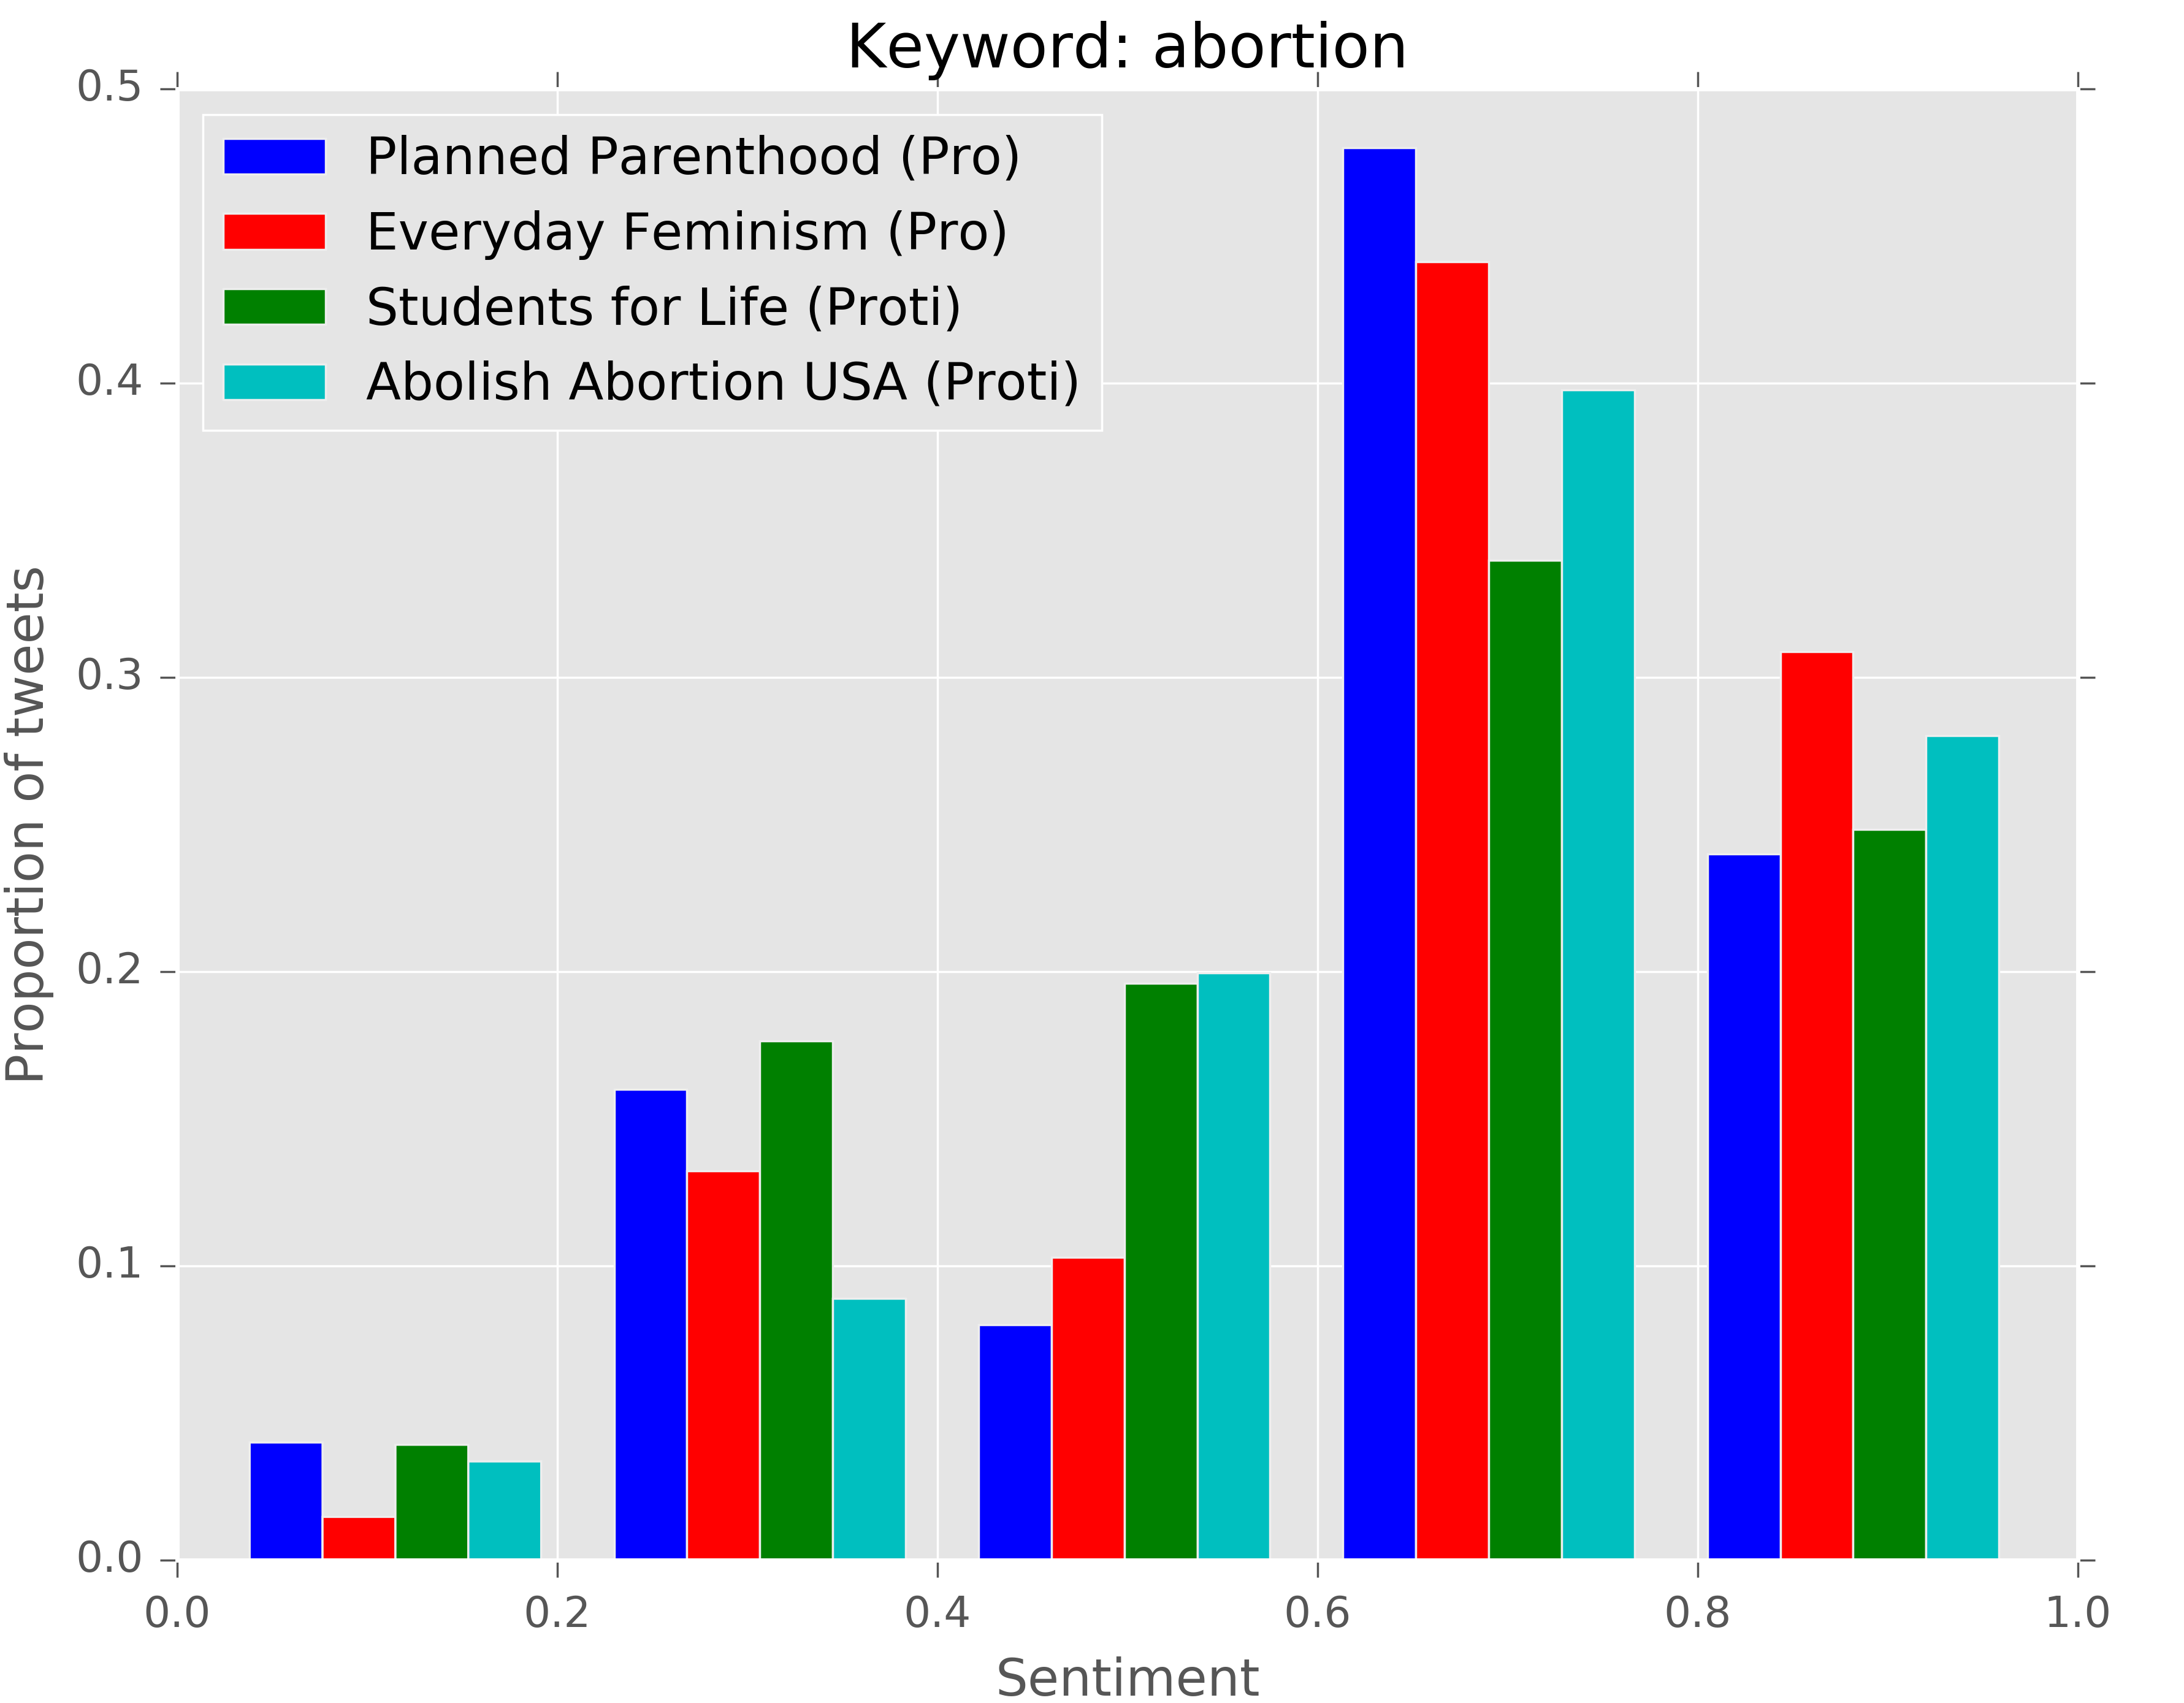
\includegraphics[scale=0.37]{./Pics/abortion-normed.png}
        \vspace{-0.2cm}
        \caption*{Normalizovaný histogram - proporce sentimentu.}
    \end{figure}
    \vspace{-0.4cm}
	\begin{itemize}
		\item proti potratu $\rightarrow$ sentiment $< 0.5$
        \item pro potrat $\rightarrow$ sentiment $> 0.5$
	\end{itemize}
\end{frame}
% ############################################
% ############################################
\begin{frame}{Future plans}
    \center
    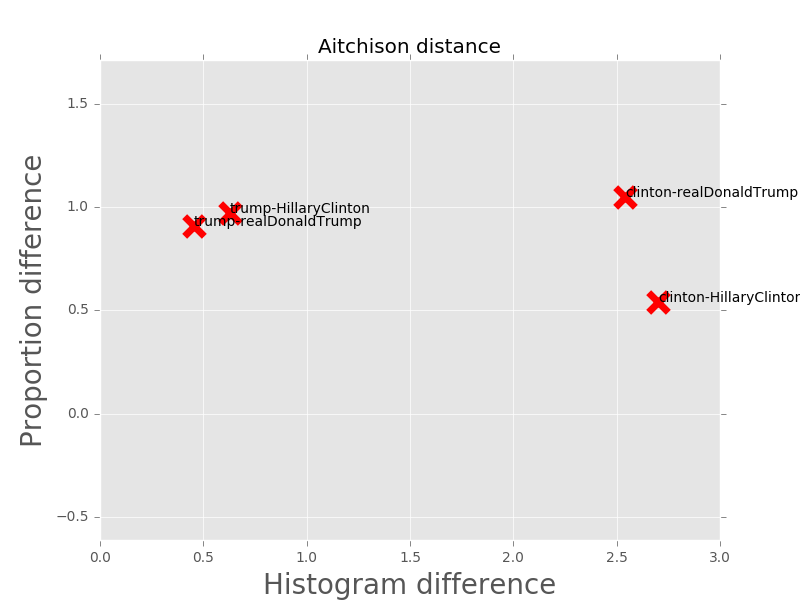
\includegraphics[scale=0.52]{./Pics/measure.png}
\end{frame}
% ############################################
% ############################################
\begin{frame}{Závěr}
    \begin{block}{Nová metoda:}
        \begin{itemize}
            \item velké množství dat - \textbf{potlačení šumu}
            \item \textbf{přímější} než tradiční výzkum
            \item první krok ke kvantitativnímu výzkumu
        \end{itemize}
    \end{block}

    \begin{block}{Měření:}
    	\begin{itemize}
            \item Trump $\rightarrow$ slabá homogenita obsahu
            \item potrat $\rightarrow$ \textbf{ohrožení} objektivity
    	\end{itemize}
    \end{block}
\end{frame}
% ############################################
% ############################################
\begin{frame}

\end{frame}
% ############################################
% ############################################
\begin{frame}{Příklady tweetů}
    \begin{block}{Everyday Feminism:}
        \begin{itemize}
            \item \begin{footnotesize} \uv{\textit{We're proud of all of the abortion providers in this room - thank you for your brave; compassionate care. \#Proud2Provide \#LifesWork}}\end{footnotesize} (0.9776)
        \end{itemize}
    \end{block}
    \begin{block}{Abolish Abortion USA:}
        \begin{itemize}
            \item \begin{footnotesize} \uv{\textit{And look at the Planned parenthood abortion rooms.....887 babies killed a day and 300,000 dead babies a year....!!!}} \end{footnotesize} (0.2255)
        \end{itemize}
    \end{block}
\end{frame}
\end{document}
